\documentclass[review,preprint,12pt]{elsarticle}
\usepackage{graphicx}
\usepackage{amssymb,amsmath}
\usepackage{subfigure}
\usepackage{makeidx}
\usepackage{booktabs,ctable,tabulary,multirow,color}
\usepackage{nomencl}
\usepackage{textcomp}
\usepackage{colortbl}

\newcommand{\varA}[1]{{\operatorname{#1}}}
\newcommand{\varB}[1]{{\operatorname{\mathit{#1}}}}

\makenomenclature

\RequirePackage{ifthen}
\renewcommand{\nomgroup}[1]{%
\ifthenelse{\equal{#1}{A}}{\item[\textbf{Roman letters}]}{%
\ifthenelse{\equal{#1}{B}}{\item[\textbf{Greek letters}]}{}}{%
\ifthenelse{\equal{#1}{C}}{\item[\textbf{Subscripts}]}{}}{%
\ifthenelse{\equal{#1}{D}}{\item[\textbf{Abbreviations}]}{}}}

\journal{Applied Thermal Engineering}

\begin{document}

\begin{frontmatter}

\title{Effect of Jet Length and Ambient Temperature on the Performance of a Two-Phase Jet Impingement Heat Sink Refrigeration System}
\author{Pablo A. de Oliveira}
\author{Jader R. Barbosa Jr.}
\ead{jrb@polo.ufsc.br}
\address{POLO Research Laboratories for Emerging Technologies in Cooling and Thermophysics, Department of Mechanical Engineering, Federal University of Santa Catarina (UFSC), Florian\'{o}polis, SC, 88040900, Brazil, Phone/Fax: (+ 55) 48 3721-7900}

\begin{abstract}

The jet impingement heat sink integrated with a compact oil-free R-134a vapor compression refrigeration system presented in a previous work \cite{OliveiraBarbosaJr.2016} is now evaluated in terms of the influence of the compressor piston stroke, applied thermal load, orifice-to-heater distance (jet length) and ambient (hot end) temperature. The proposed heat sink is a compact active thermal solution for concentrated heat loads as it integrates the evaporator and the expansion device into a single unit, making use of a single two-phase impinging jet as the cooling mechanism. The present analysis is based on the coefficient of performance and other steady-state heat transfer parameters associated with the impinging jet (heat transfer coefficient and heater surface temperature). A reduction of the jet length promoted a more vigorous splattering of the jet on the heated surface, enhancing the droplet breakup, which in turn reduced significantly the critical heat flux. An increase of the hot reservoir temperature increased the jet impingement heat transfer coefficient.

\end{abstract}

\end{frontmatter}

\vspace{0.5cm}

\noindent {\bf Keywords:} Jet impingement, vapor compression, compact system, oil-free compressor, electronics cooling.

\printnomenclature[1.4cm]

\pagebreak

\section{Introduction}

Advances in the design and micro-fabrication of electronic devices have led to a continual scale reduction of circuit components, which increased the number of \textcolor{blue}{heat sources per unit volume and, consequently, the heat dissipation} per unit surface area \cite{Bar-Cohen2014}. As temperature \textcolor{blue}{is responsible for} more than 50\% of \textcolor{blue}{known causes of} failure \cite{Anandan2008}, thermal management is of utmost importance \textcolor{blue}{to the} reliability and \textcolor{blue}{safe operation} of electronic devices. To date, several cooling technologies \textcolor{blue}{have been studied with a focus on} a variety of \textcolor{blue}{applications}, such as advanced military avionics, \textcolor{blue}{high-power lasers}, high-performance computers, hybrid/electric vehicles, mobile devices and data servers \cite{Mudawar2001,Chu2004,Nakayama2009,HangKabbani2015,KheirabadiGroulx2016}.

Passive cooling technologies, i.e., those that do not rely on refrigeration, may employ {\it indirect liquid cooling} \textcolor{blue}{in such a way that the cooling performance is partially determined by the convective heat transfer of} a liquid coolant flowing through the thermal management device (finned heat sink, heat pipe or cold plate). Nevertheless, the performance also depends on the thermal resistances of the different layers of materials separating the electronic device from the liquid coolant, which \textcolor{blue}{results in} a relatively large temperature gradient when high heat fluxes \textcolor{blue}{are dissipated}. These thermal resistances can be eliminated by {\it direct liquid cooling} of the electronic component \cite{Bar-Cohen2006}. Direct liquid cooling is advantageous only when its convective thermal resistance is smaller than the sum of the convective, conductive and contact resistances of  indirect liquid cooling. Because heat spreading plays a minor role in a direct cooling system, high-heat-flux components may be packaged quite close to one another, greatly reducing both the weight and the volume of the cooling system \cite{Mudawar2008}. However, bringing the coolant into direct contact with the surface of the heat spreader, or \textcolor{blue}{with} the electronic component itself, limits the options to a few dielectric \textcolor{blue}{fluids} \cite{Mudawar2008,Starke2005}. Given the inferior thermophysical properties of dielectric \textcolor{blue}{fluids} and the strong dependence of cooling performance on convective resistance, the viability of a direct cooling system is highly dependent on \textcolor{blue}{its} ability to \textcolor{blue}{produce very high} convective heat transfer coefficients. \textcolor{blue}{S}prays and jets in convective boiling \textcolor{blue}{are highly effective cooling schemes} due to their enhanced heat transfer coefficients and  nonlinear relationship between heat flux and surface-to-fluid temperature difference \cite{Sung2009a}. Cooling solutions that rely on two-phase flow heat transfer, such as sprays, jets and boiling in microchannels have been \textcolor{blue}{extensively} investigated \textcolor{blue}{in the literature} \cite{Bar-Cohen2006,Agostini2007,Kandlikar2007,Ebadian2011,Marcinichen2013,Kadam2014,Cheng2016,RiofrioCaneyGruss2016,SmakulskiPietrowicz2016}. 

\textcolor{blue}{Integration of vapor compression systems with  two-phase heat transfer schemes is an innovative and effective way of removing highly concentrated heat loads \cite{OliveiraBarbosaJr.2016,BarbosaJr.2012,Trutassanawin2006,MarcinichenThomeMichel2010}.} However, the majority of the direct-liquid cooling systems  \textcolor{blue}{proposed in the literature} do not operate in a mechanical vapor compression circuit \cite{Whelan2012,Wang2011a,Browne2012,Parida2012,Buchanan2013,Joshi2015,Maddox2015,Gould2015}. A few exceptions used spray cooling as the heat transfer technique, \textcolor{blue}{but were not purposely designed to be compact or miniaturized} \cite{Yan2010,Tan2013,Xie2014,Chunqiang2012,Xu2014,Hou2015,Chen2015}. \textcolor{blue}{Oil lubricated compressors}  \cite{Chunqiang2012,Xu2014,Hou2015,Chen2015}, ancillary expansion valves \cite{Yan2010,Tan2013,Chunqiang2012,Xu2014} and tube evaporators \cite{Hou2015,Chen2015} were \textcolor{blue}{often needed} to operate the active cooling system.    

As far as the present authors are aware, an active cooling system that integrates two-phase impinging jets and mechanical vapor compression refrigeration has not yet been reported in the literature. The present paper \textcolor{blue}{extends} the performance evaluation of the compact refrigeration system introduced in Ref.~\cite{OliveiraBarbosaJr.2016}. The main component of this system is a thermal management module that combines a micro-orifice as the expansion device and a jet-impingement-based evaporator/heat sink into a single cooling unit, which is capable of dissipating high heat loads and providing \textcolor{blue}{the} full expansion required by the refrigerant \textcolor{blue}{to achieve the desired evaporating temperature}. The full potential size reduction \textcolor{blue}{of the system} is \textcolor{blue}{complemented with} the use of a linear small-scale oil-free R-134a compressor. 

The experimental \textcolor{blue}{performance analysis presented in this paper} focuses on the influence of the compressor piston stroke, applied thermal load, orifice-to-heater distance and hot reservoir (ambient) temperature. The \textcolor{blue}{main output performance parameters are} the coefficient of performance and on steady-state heat transfer parameters associated with the impinging jet \textcolor{blue}{(heat transfer coefficient and heater surface temperature)}.

\section{Experimental Work}

\subsection{Experimental Apparatus}
\label{sec:Experimental_Apparatus}

\textcolor{blue}{The experimental apparatus shown in Fig.~\ref{fig:Figure_1} has been presented in detail in Ref.~\cite{OliveiraBarbosaJr.2016}, so only the main features will be presented here}. A small-scale (0.27 cm$^{3}$ maximum volumetric displacement, 340 Hz operating frequency, 1.3 kg total weight) R-134a oil-free linear-motor compressor was used. The compressor was equipped with a frequency inverter to control the volumetric displacement (piston stroke). A digital power meter was employed to measure the electrical power consumption of the compressor.  %The compressor was positioned inside a purpose-built calorimeter which was developed to indirectly measure the heat dissipation rate through the compressor shell, thus providing closure for the overall system energy balance. The apparatus was insulated with elastomeric foam to prevent thermal leaks to the surroundings \cite{Oliveira2016}. 
\textcolor{blue}{The temperature of the hot reservoir (ambient) was controlled by a} brazed plate counter-flow liquid-cooled condenser.

\begin{figure}[htp!]
\centering
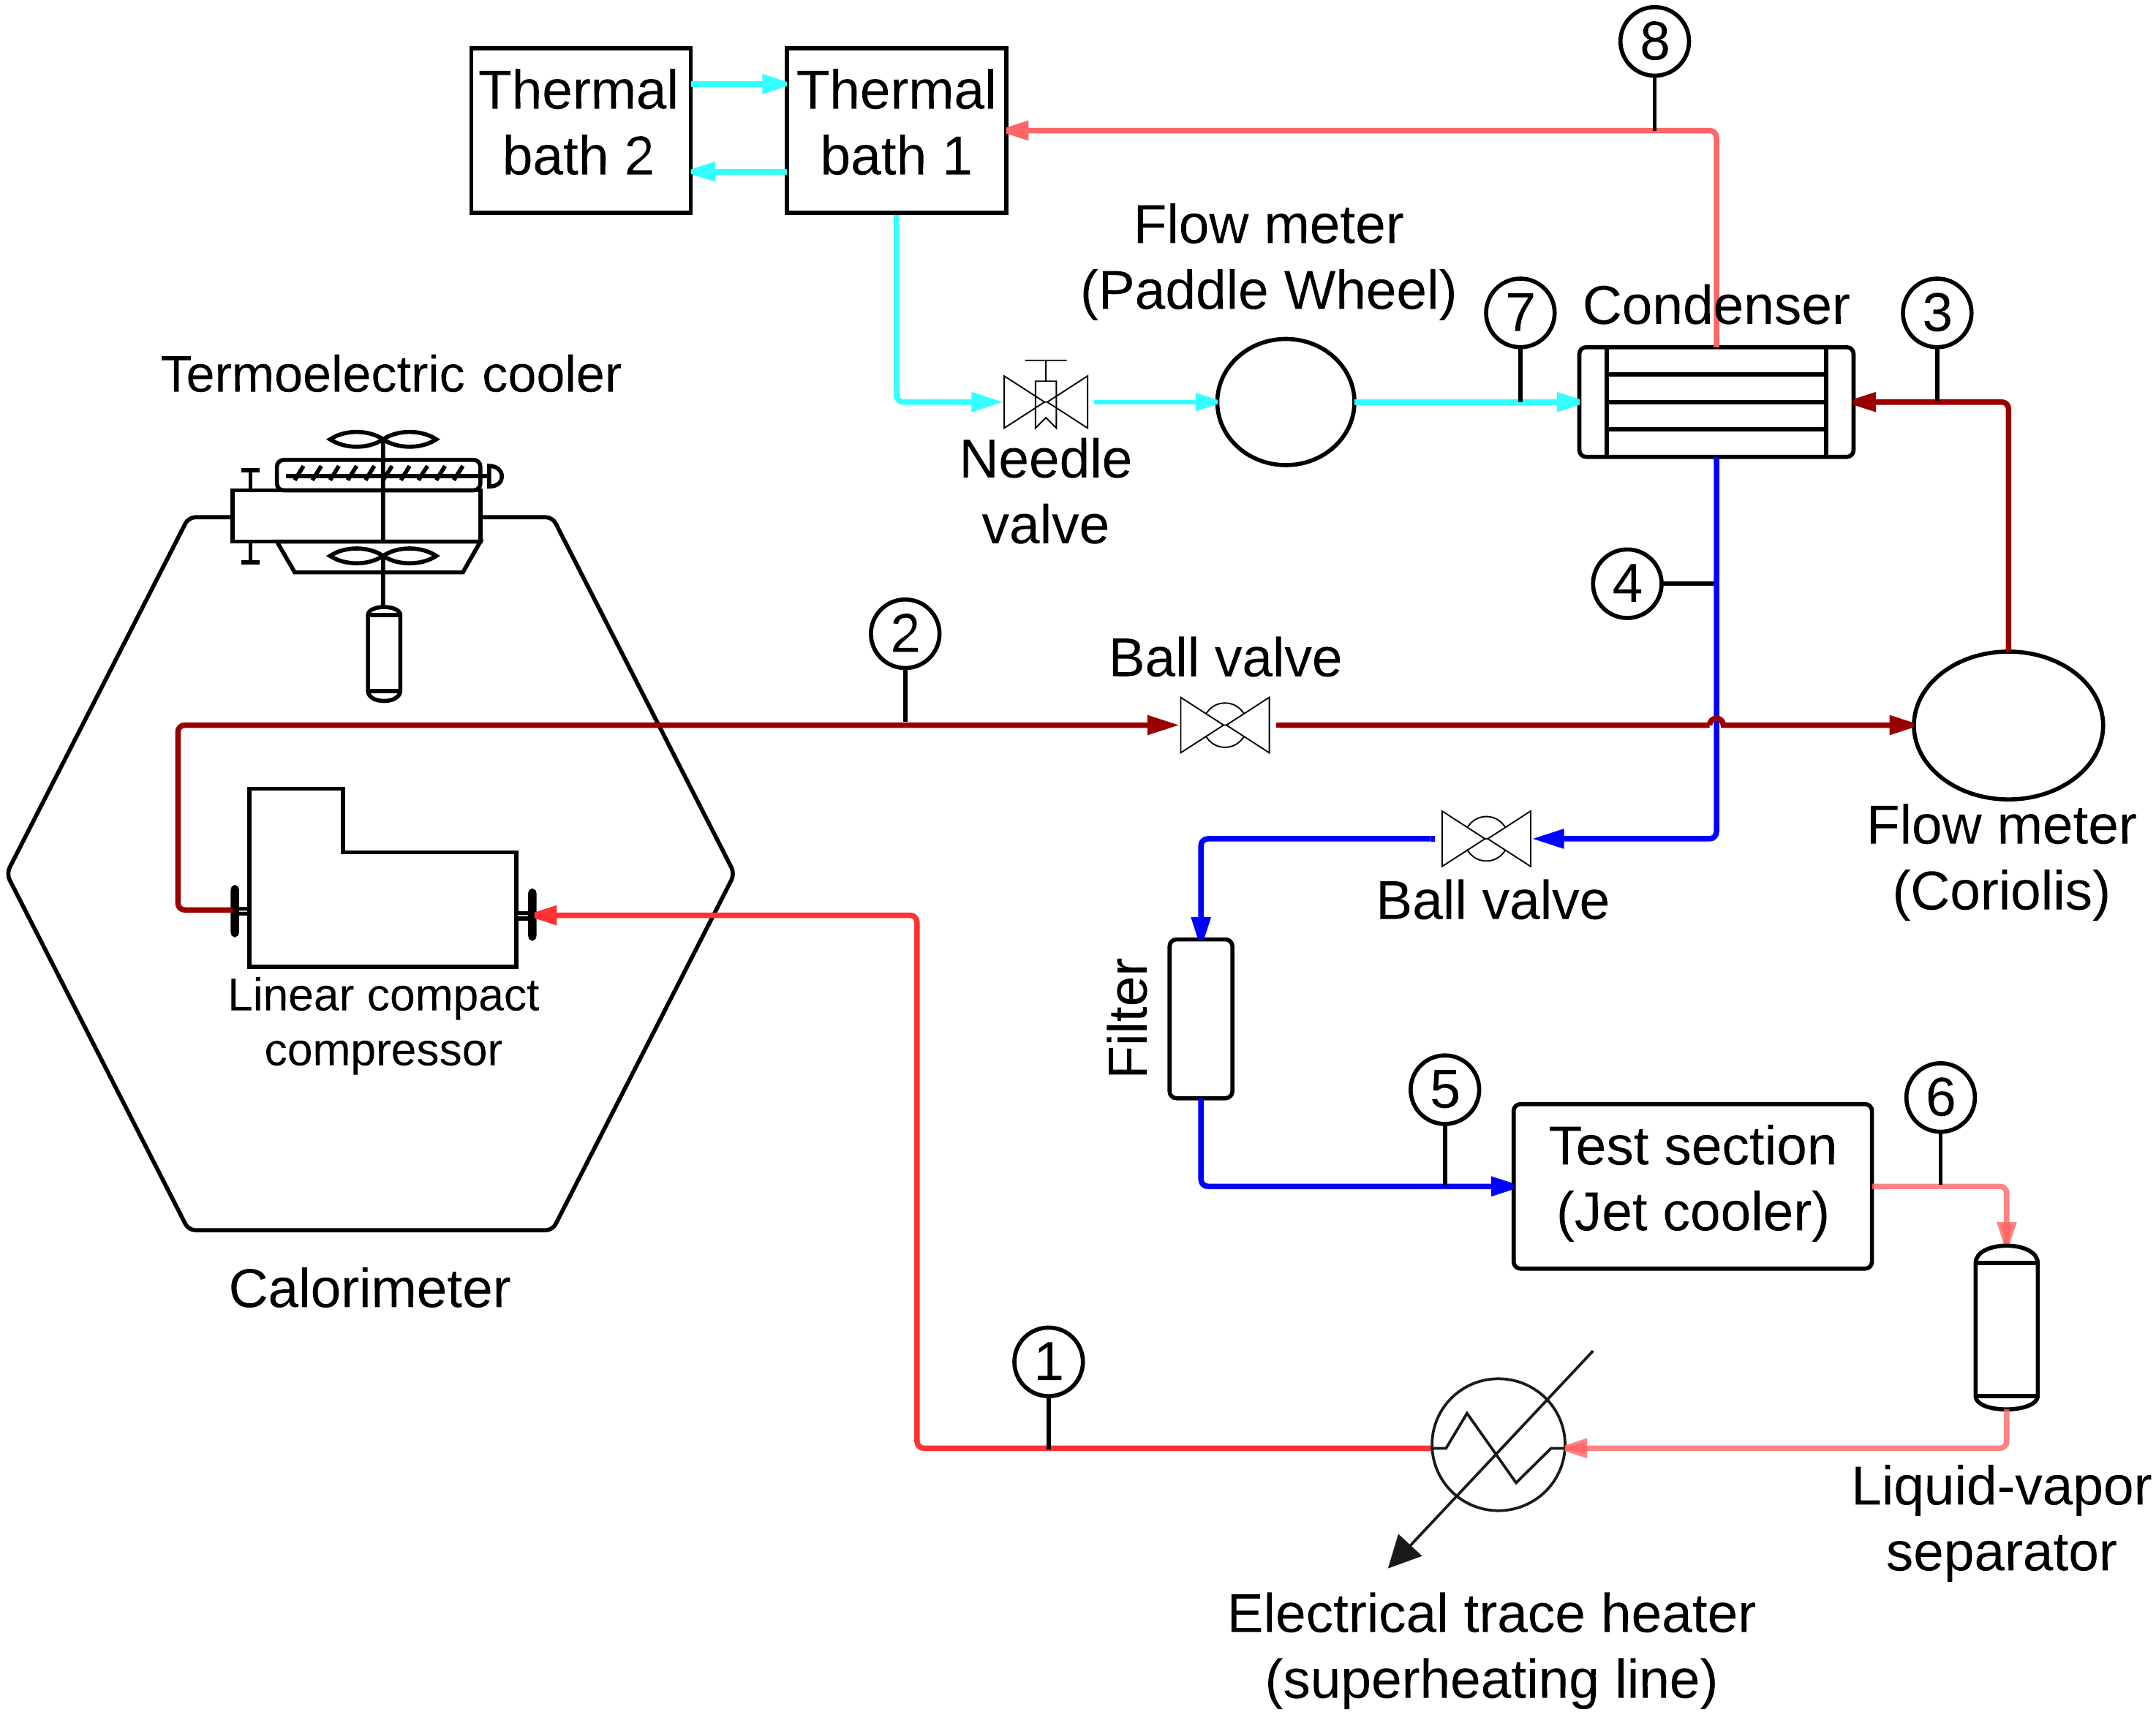
\includegraphics[angle=0,scale=0.4]{Figure_1.png}
\caption{Schematic diagram of the experimental apparatus: (1) Compressor inlet (suction); (2) Compressor outlet (discharge); (3) Condenser inlet (refrigerant side); (4) Condenser outlet (refrigerant side); (5) Jet cooler inlet; (6) Jet cooler outlet; (7) Condenser inlet (WEG side); (8) Condenser outlet (WEG side).}
\label{fig:Figure_1}
\end{figure}

A Coriolis mass flow meter (uncertainty of $\pm$ 0.05 kg/h) was \textcolor{blue}{used} to measure the R-134a mass flow rate. The volumetric flow rate of the \textcolor{blue}{condenser coolant} --- a 90\%/10\% vol.~mixture of distilled water and ethylene glycol (WEG) --- was measured with a paddle wheel flow meter (uncertainty of $\pm$ 0.07 L/min). Absolute pressure transducers (uncertainties of $\pm$ 0.05 bar and $\pm$ 0.03 bar for the high- and low-pressure sides, respectively) and resistance temperature detectors (uncertainty of $\pm$ 0.20\textcelsius) were used to measure the local pressures and temperatures (and monitor in real time the thermodynamic states of the \textcolor{blue}{refrigerant}) at the points shown in Fig.~\ref{fig:Figure_1}. 

\nomenclature[DWEG]{WEG}{Water-Ethylene Glycol}%

\textcolor{blue}{The refrigerant may leave the test section (two-phase jet heat sink) with a significant liquid fraction, which is needed to maintain a high overall thermal conductance of the unit \cite{OliveiraBarbosaJr.2016}. Therefore, an electrical trace heater wrapped around the compressor suction line was installed to guarantee a safe operation of the compressor.} In a lab test device such as the present apparatus, Joule heating is \textcolor{blue}{easier to} supply and control. However, in a real application, the superheating thermal energy may come from an internal heat exchanger  \textcolor{blue}{(using the condenser as a heat source)}, not necessarily adding to the electrical supply to the system. The temperature of point 1 (compressor inlet in Fig.~\ref{fig:Figure_1}) was accurately controlled so as to maintain a fixed refrigerant superheating degree at the compressor inlet. The complete specification of setup components, measurement instrumentation and variable control strategies can be found in Refs.~\cite{OliveiraBarbosaJr.2016,Oliveira2016}.


\subsection{Two-Phase Jet Heat Sink}
\label{sec:Jet_Cooler}

The novel heat sink combines the expansion device and the evaporator into a single cooling module using a two-phase imping\textcolor{blue}{ing} jet to remove \textcolor{blue}{the} heat load from a small surface. The assembly of the two-phase jet heat sink in the experimental setup is presented in Fig.~\ref{fig:Figure_2}. The jet cooler is composed of a metallic cap, a \textcolor{blue}{polycarbonate} jet impingement chamber, an internal orifice plenum, a polymeric unit that serves for thermal insulation and fluid drainage, a reservoir to collect the  \textcolor{blue}{outlet} two-phase mixture, a film heater and a copper block that emulates the electronic component. 

This study explores two versions of the jet cooler, which differ \textcolor{blue}{in} the\textcolor{blue}{ir} jet chamber heights. In both versions, the external dimensions are 80 mm (width) $\times$ 80 mm (depth) and the heights are 112.5 mm and 93.5 mm for Figs.~\ref{fig:Figure_2} (a) and (b), respectively. Fig.~\ref{fig:Figure_2} (b) shows the \textcolor{blue}{pressure and temperature} instruments to determine the thermodynamic state of the refrigerant at the inlet and outlet of the jet cooler and the RTDs used to estimate the heated surface temperature.

\nomenclature[DRTD]{RTD}{Resistance Temperature Detector}%

\begin{figure}[!h]
\centering
\subfigure[a][]{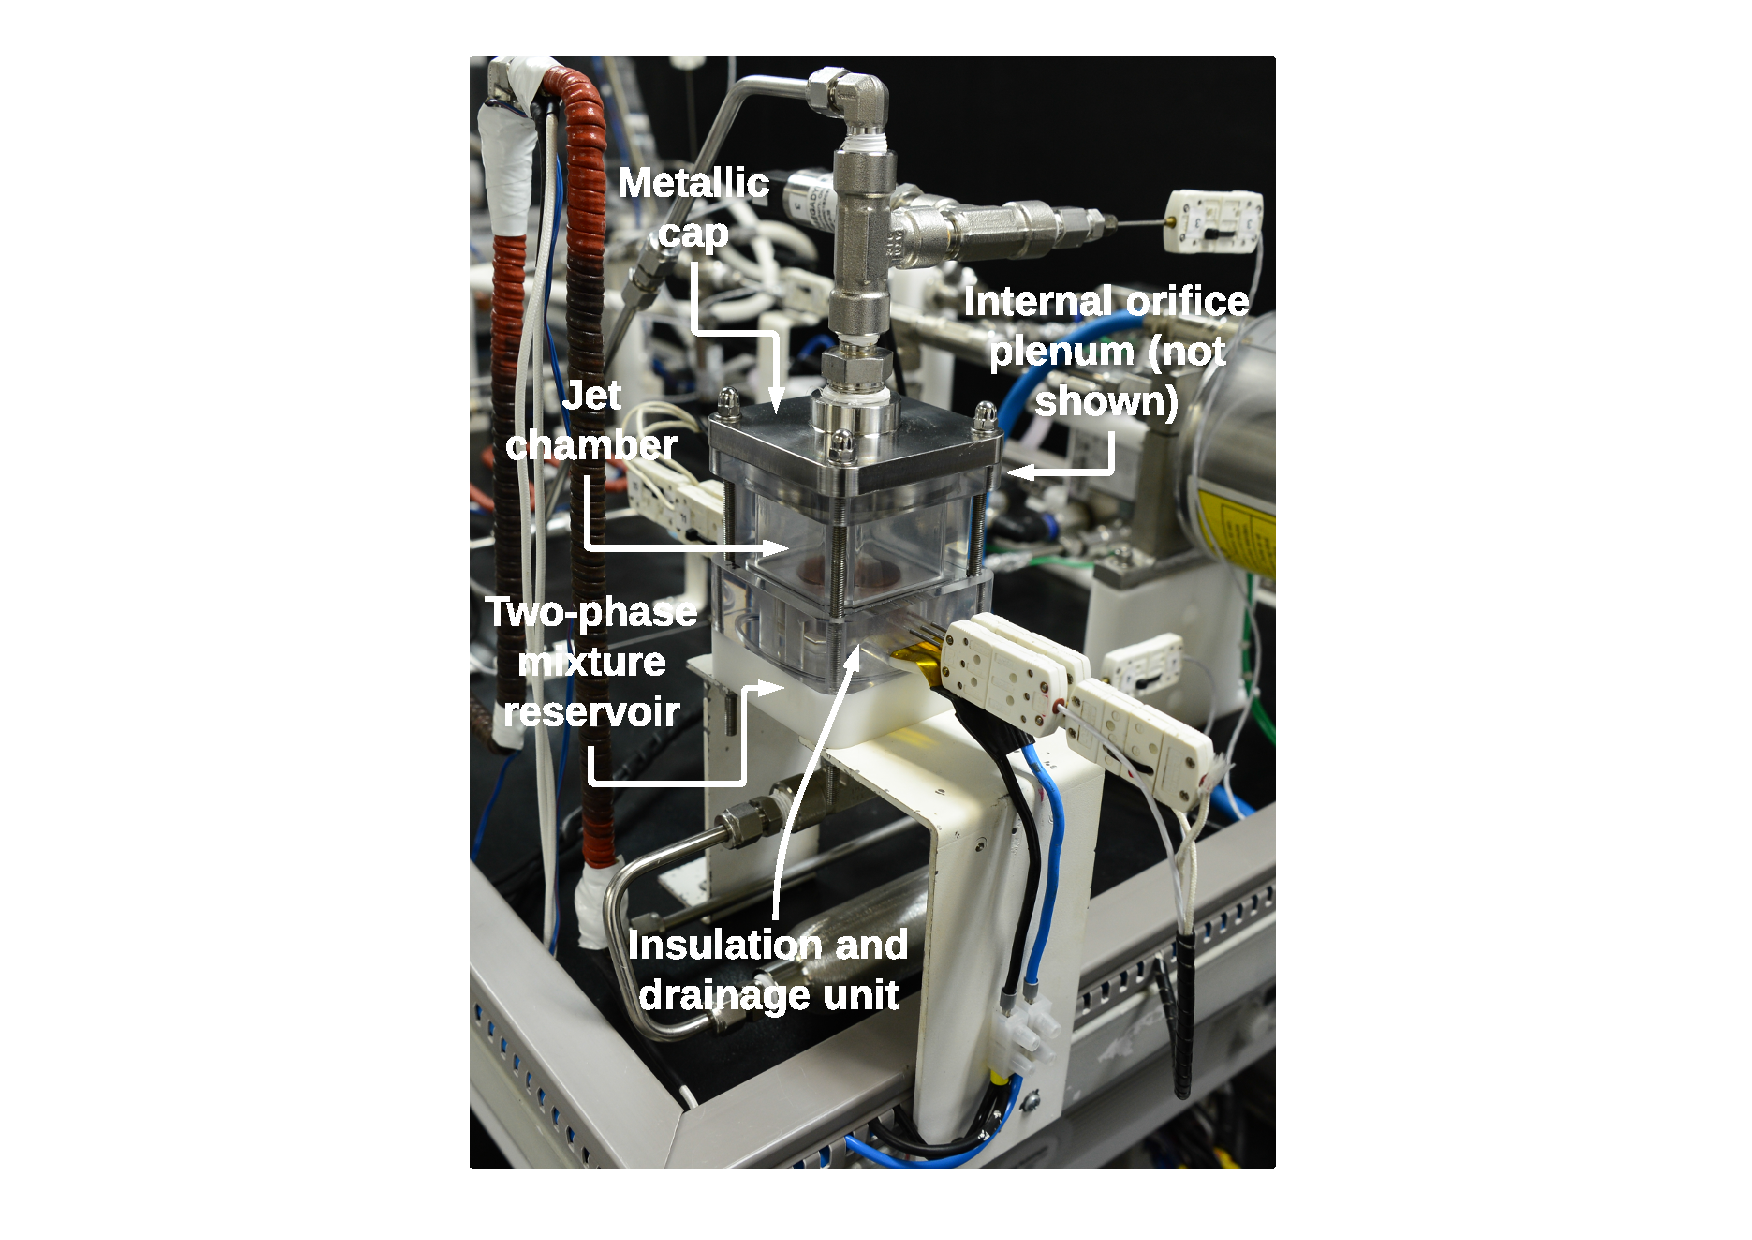
\includegraphics[angle=0,scale=0.47]{Figure_2(a).pdf}}
\hfil
\subfigure[b][]{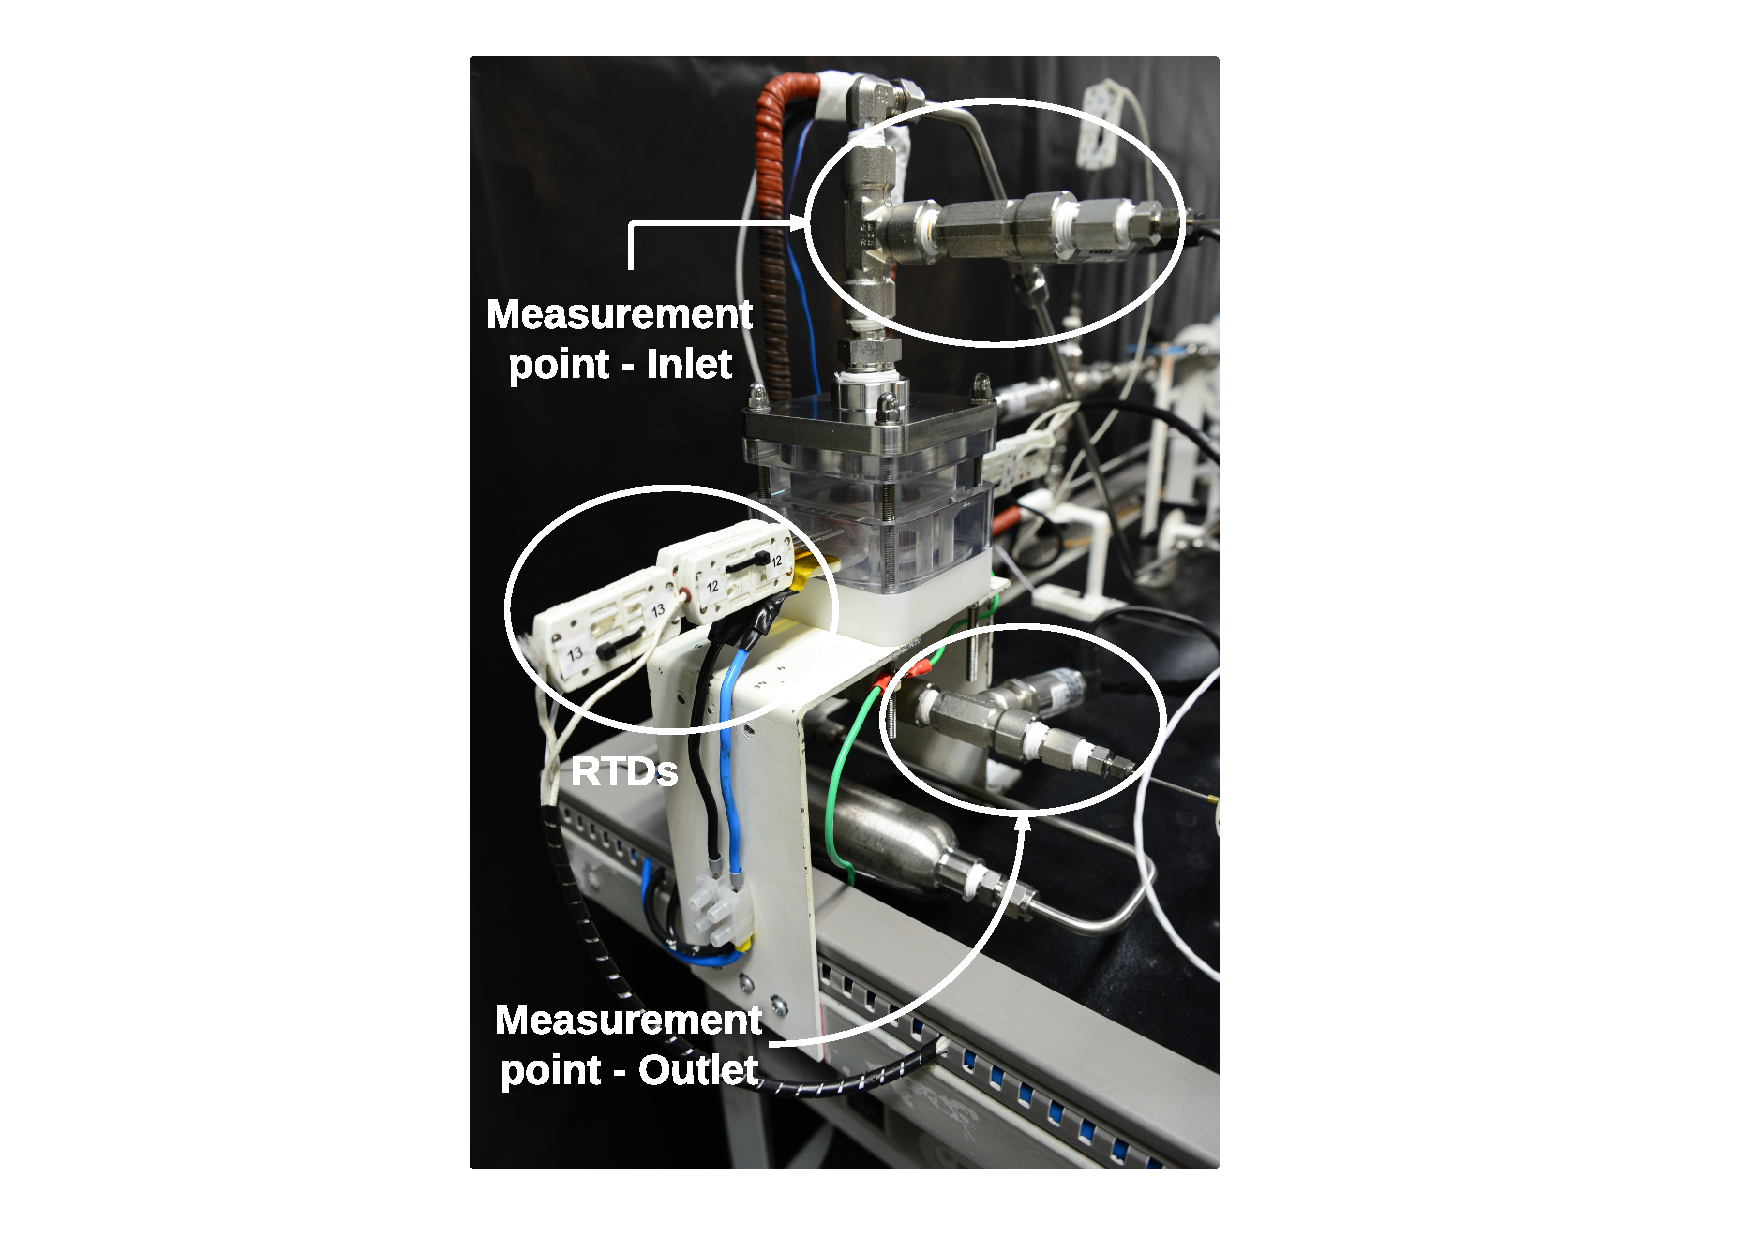
\includegraphics[angle=0,scale=0.47]{Figure_2(b).pdf}}
\caption{Two-phase jet coolers: assembly and main components. (a) 112.5-mm jet cooler, (b) 93.5-mm jet cooler}
\label{fig:Figure_2}
\end{figure} 

High-pressure sub-cooled liquid from the condenser flows through the metallic cap directly into the orifice plenum. The plenum, depicted in Fig.~\ref{fig:Figure_3} (a), comprises an AISI 316 stainless steel outer orifice plate, a polyacetal resin (POM) inner orifice plate and the expansion device, which is an array of POM 10-mm long threaded screws with the actual orifices drilled along their center lines -- see Fig.~\ref{fig:Figure_3} (b). The screws hold the orifice plates together. The plenum can accommodate up to 13 orifices in a staggered array covering a 20-mm side square area. %Before expansion, thermal losses reduction from the refrigerant to the surroundings (inner orifice plate and screws) benefit from the low thermal conductivity of POM \cite{Oliveira2016}. 
In the present study, only single-jet tests are reported. In these tests, a \textcolor{blue}{300-$\mu$m} orifice screw was positioned at the center of the orifice plate assembly and dummy screws occupied the remaining positions, as shown in Fig.~\ref{fig:Figure_4} (a). 


\nomenclature[DPOM]{POM}{Polyoxymethylene}%

\begin{figure}[!htp]
\centering
\subfigure[a][]{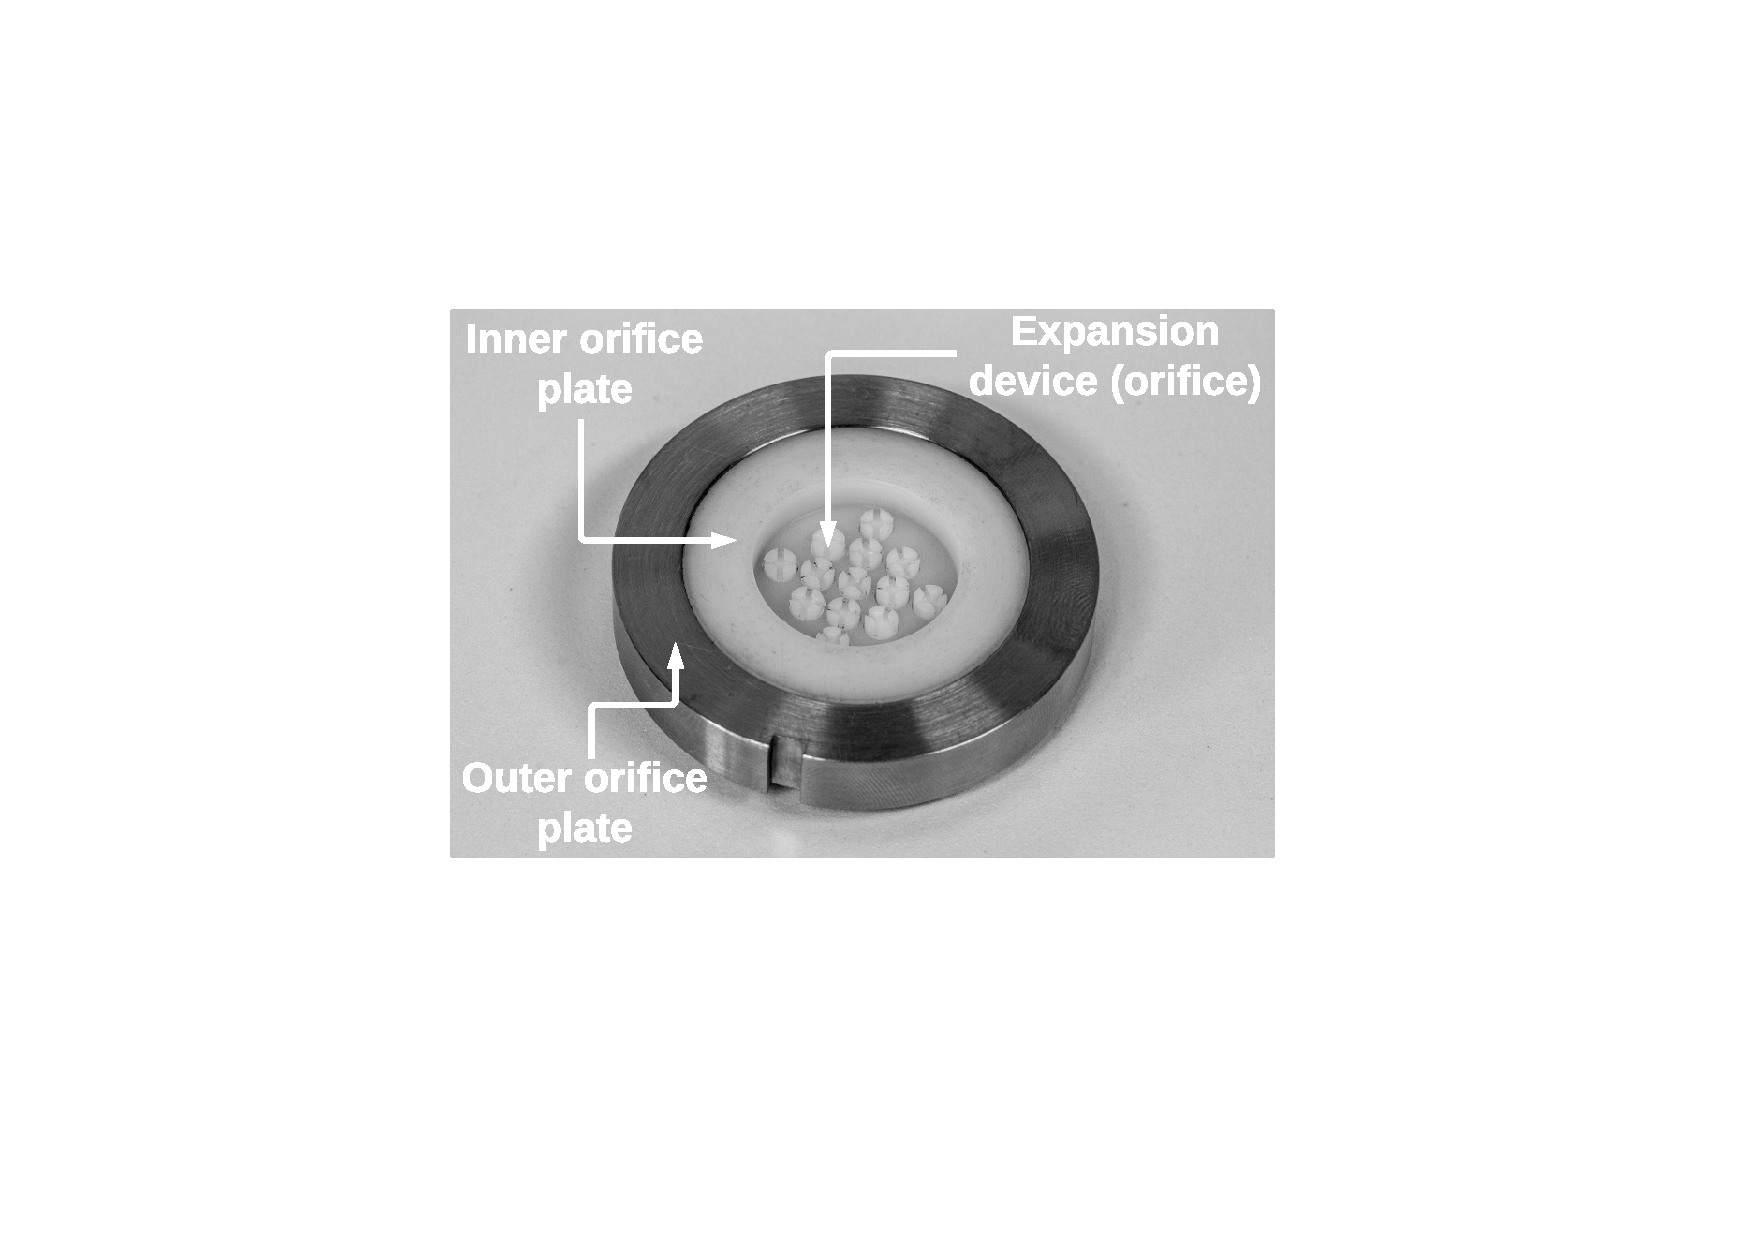
\includegraphics[angle=0,scale=0.45]{Figure_3(a).pdf}}
\hfil
\subfigure[b][]{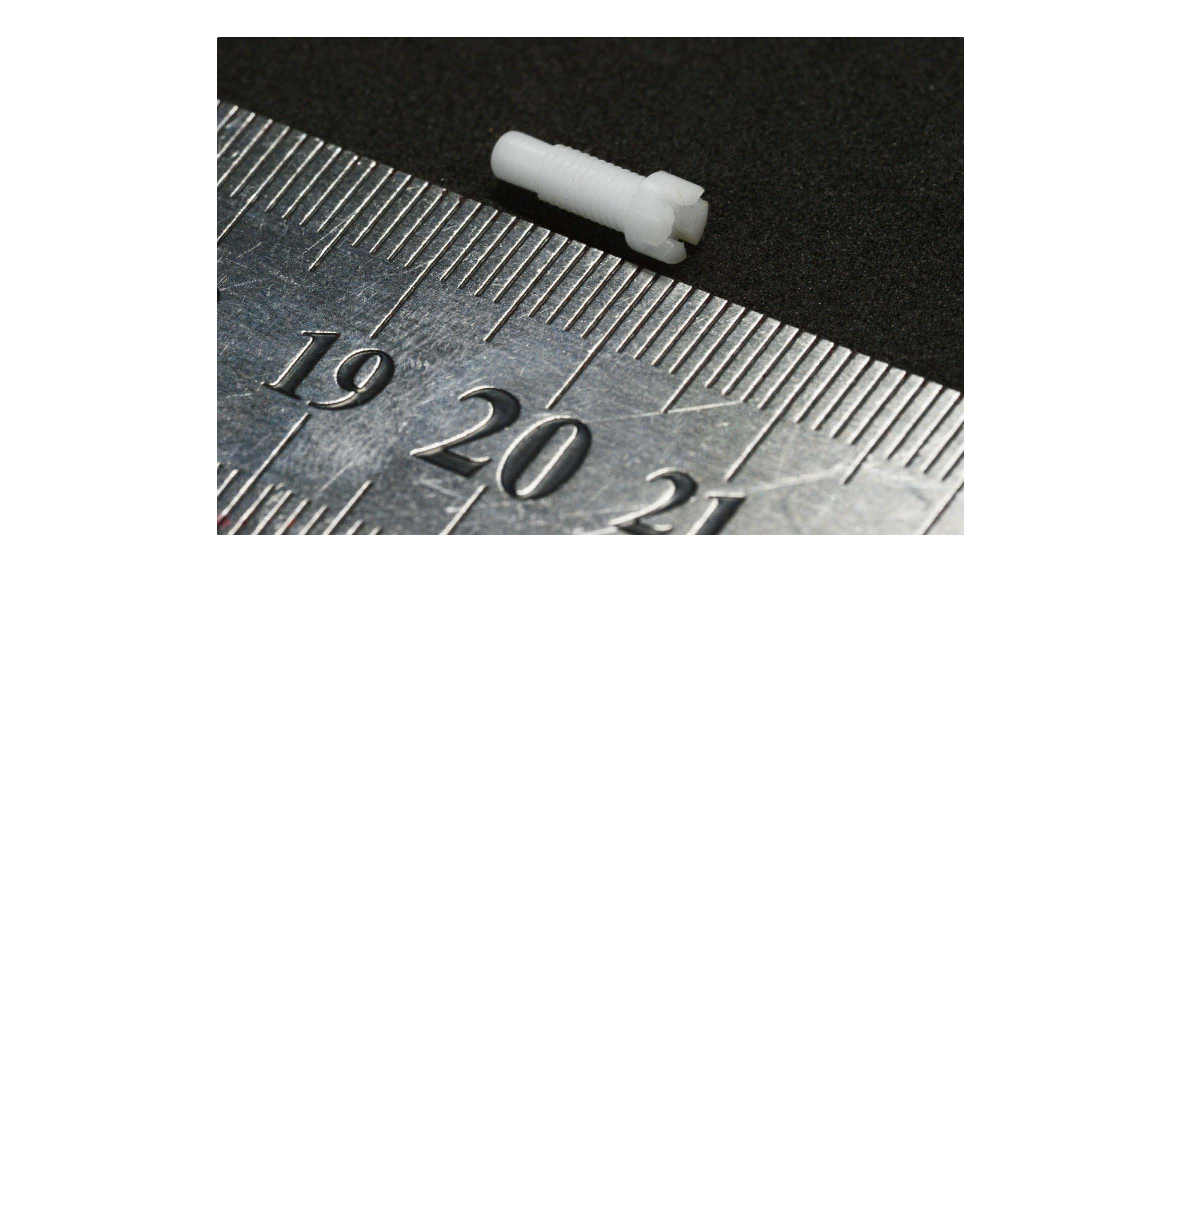
\includegraphics[angle=0,scale=0.5]{Figure_3(b).pdf}}
\caption{Orifice plenum: (a) assembled components and (b) expansion device ( \textcolor{blue}{threaded screw with an internal} orifice).}
\label{fig:Figure_3}
\end{figure} 


As the sub-cooled liquid passes through the nozzle it expands generating a downward-oriented jet inside the jet chamber. \textcolor{blue}{The values of jet length, $H$, corresponding to the two jet chambers are} $H = 28.84$  and $H = 9.75$ mm, as shown in Fig.~\ref{fig:Figure_4} (b). The jet length, i.e., the height of the chamber, is the vertical distance from the outlet of the orifice to the base of the chamber, which is at the same level of the impingement surface.

\begin{figure}[!h]
\centering
\subfigure[a][]{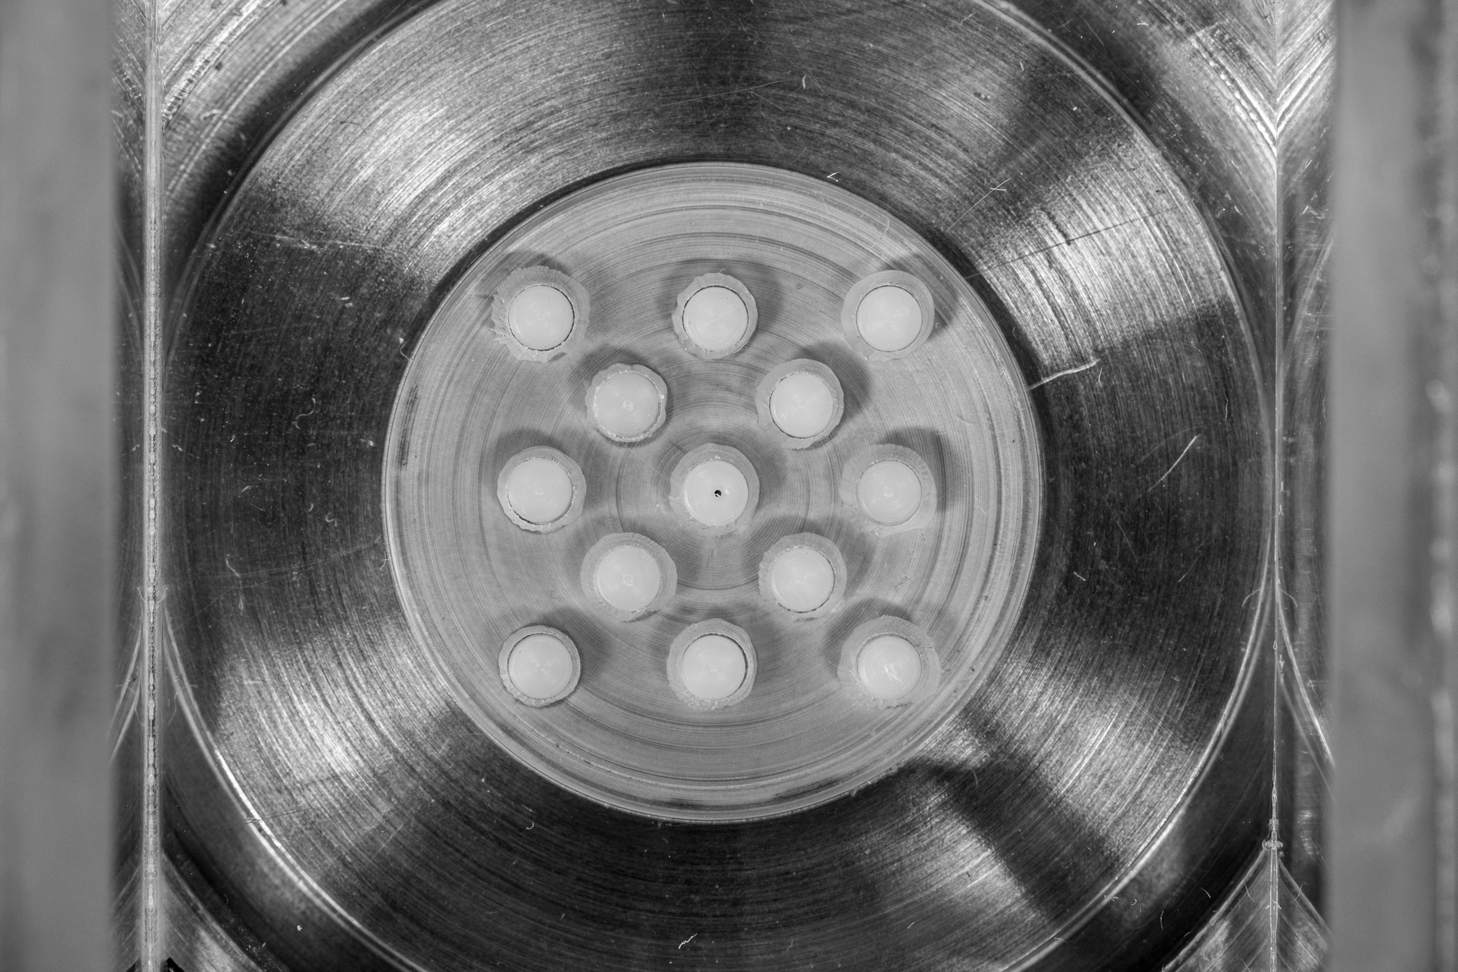
\includegraphics[angle=0,scale=0.27]{Figure_4(a).pdf}}
\hfil
\subfigure[b][]{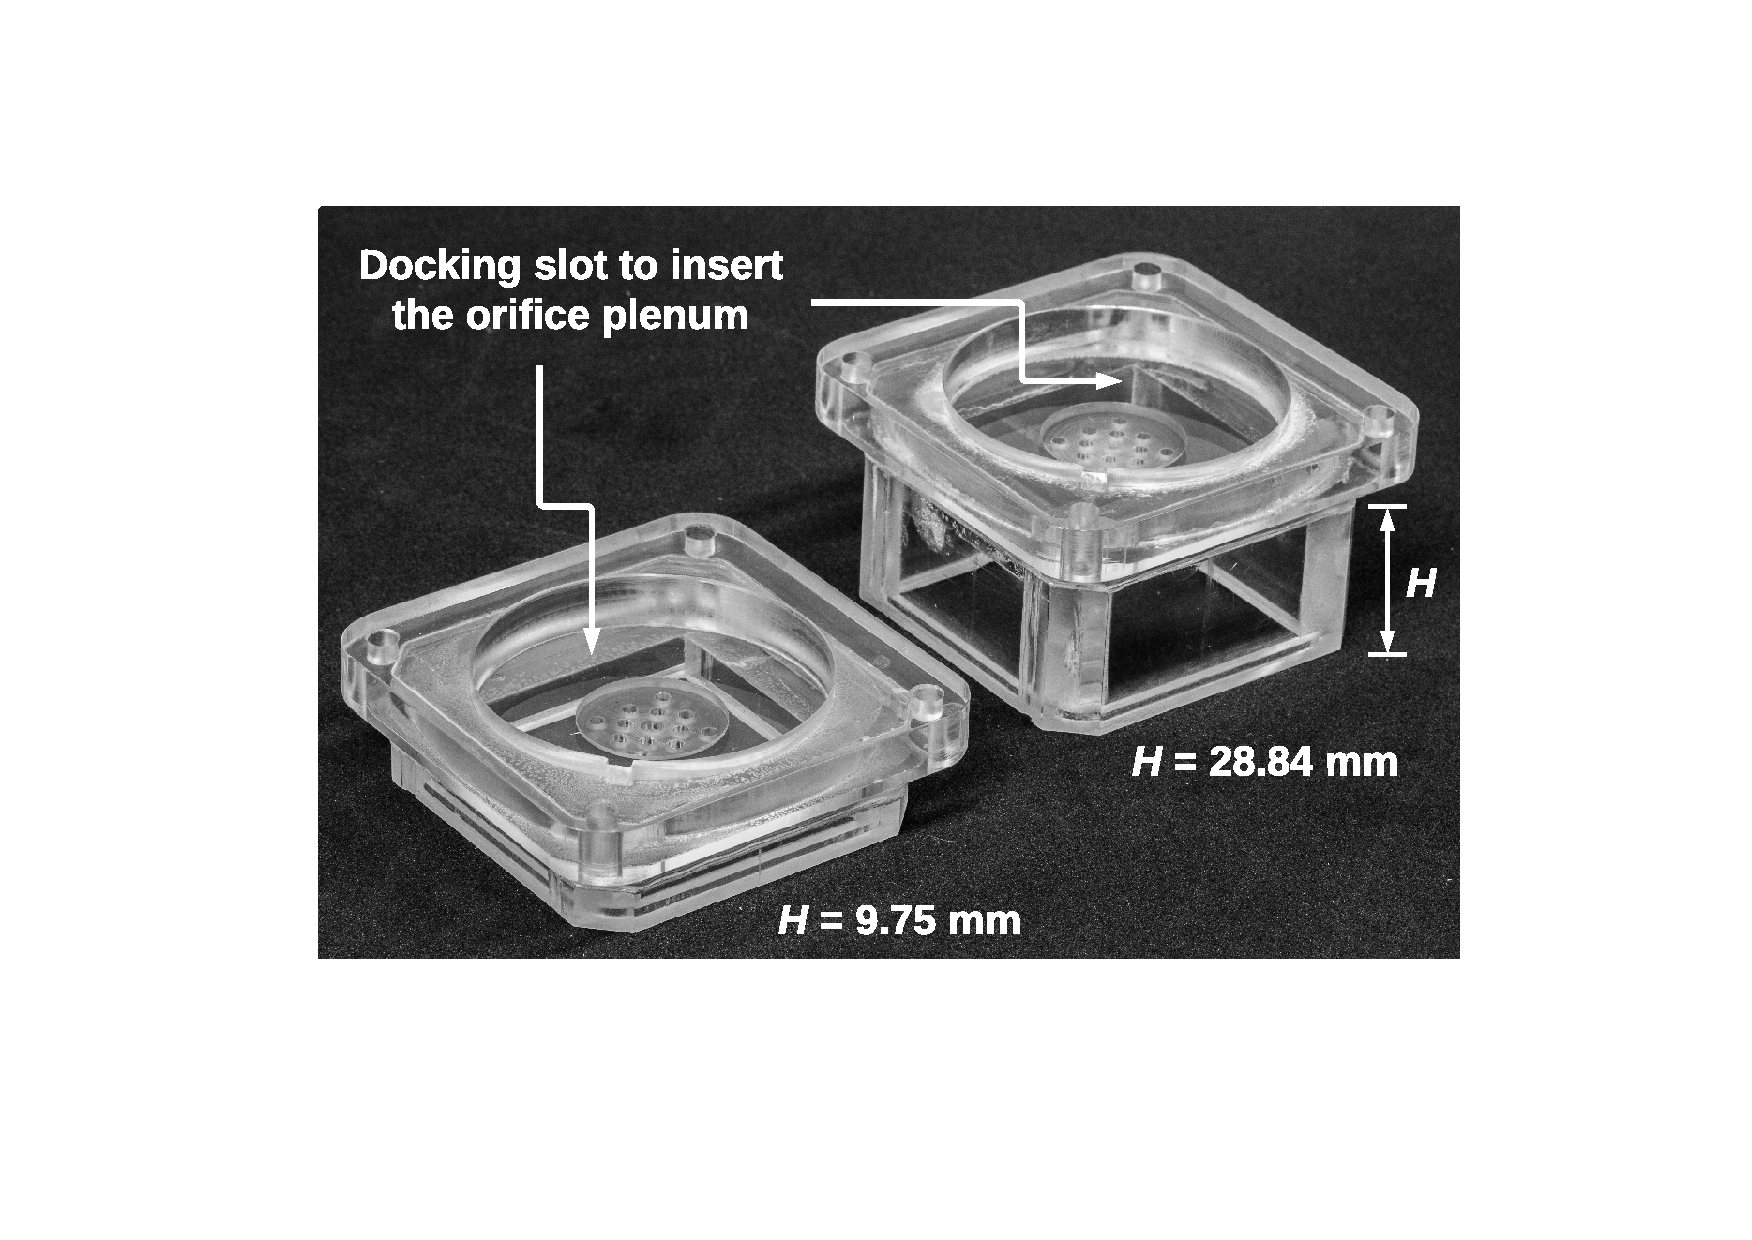
\includegraphics[angle=0,scale=0.35]{Figure_4(b).pdf}}
\caption{(a) Bottom view of the orifice plenum assembled in the jet chamber (300-$\mu$m orifice in the center). (b) Two jet chambers with different jet lengths.}
\label{fig:Figure_4}
\end{figure} 

The impingement surface is the top surface of a heated cylindrical copper block mounted in a plastic bottom piece (insulation and drainage unit) designed to thermally insulate the sides and the bottom of the copper block and facilitate drainage of the two-phase mixture from the jet chamber into the reservoir. The heat source is a 200-W skin (thin film) heater \textcolor{blue}{pressed tightly against (and in good thermal contact with) the bottom} of the copper block \textcolor{blue}{by a teflon base plate, as seen in Fig.~\ref{fig:Figure_5} (a)} \cite{OliveiraBarbosaJr.2016}. The thermal load was finely controlled by a DC digital power supply. During the experimental runs, the thermal load was increased  \textcolor{blue}{in steps} by increasing the voltage or the current provided by the power supply. The copper block has six RTD wells, as shown in Fig.~\ref{fig:Figure_5} (b). Five RTDs are used to measure the temperature and allow for an estimate of the surface temperature to be made using Fourier's law. The remaining one is connected to a commercial PID controller that functions as a safety system cutting the heating power supply in the event of a temperature runaway associated with the critical heat flux. The area of the target surface is 6.36 cm$^{2}$ ($D$ = 28.54 mm) and the distance from the plane of the RTDs to the impingement surface is 10.03 mm.

\begin{figure}[!htp]
\centering
\subfigure[a][]{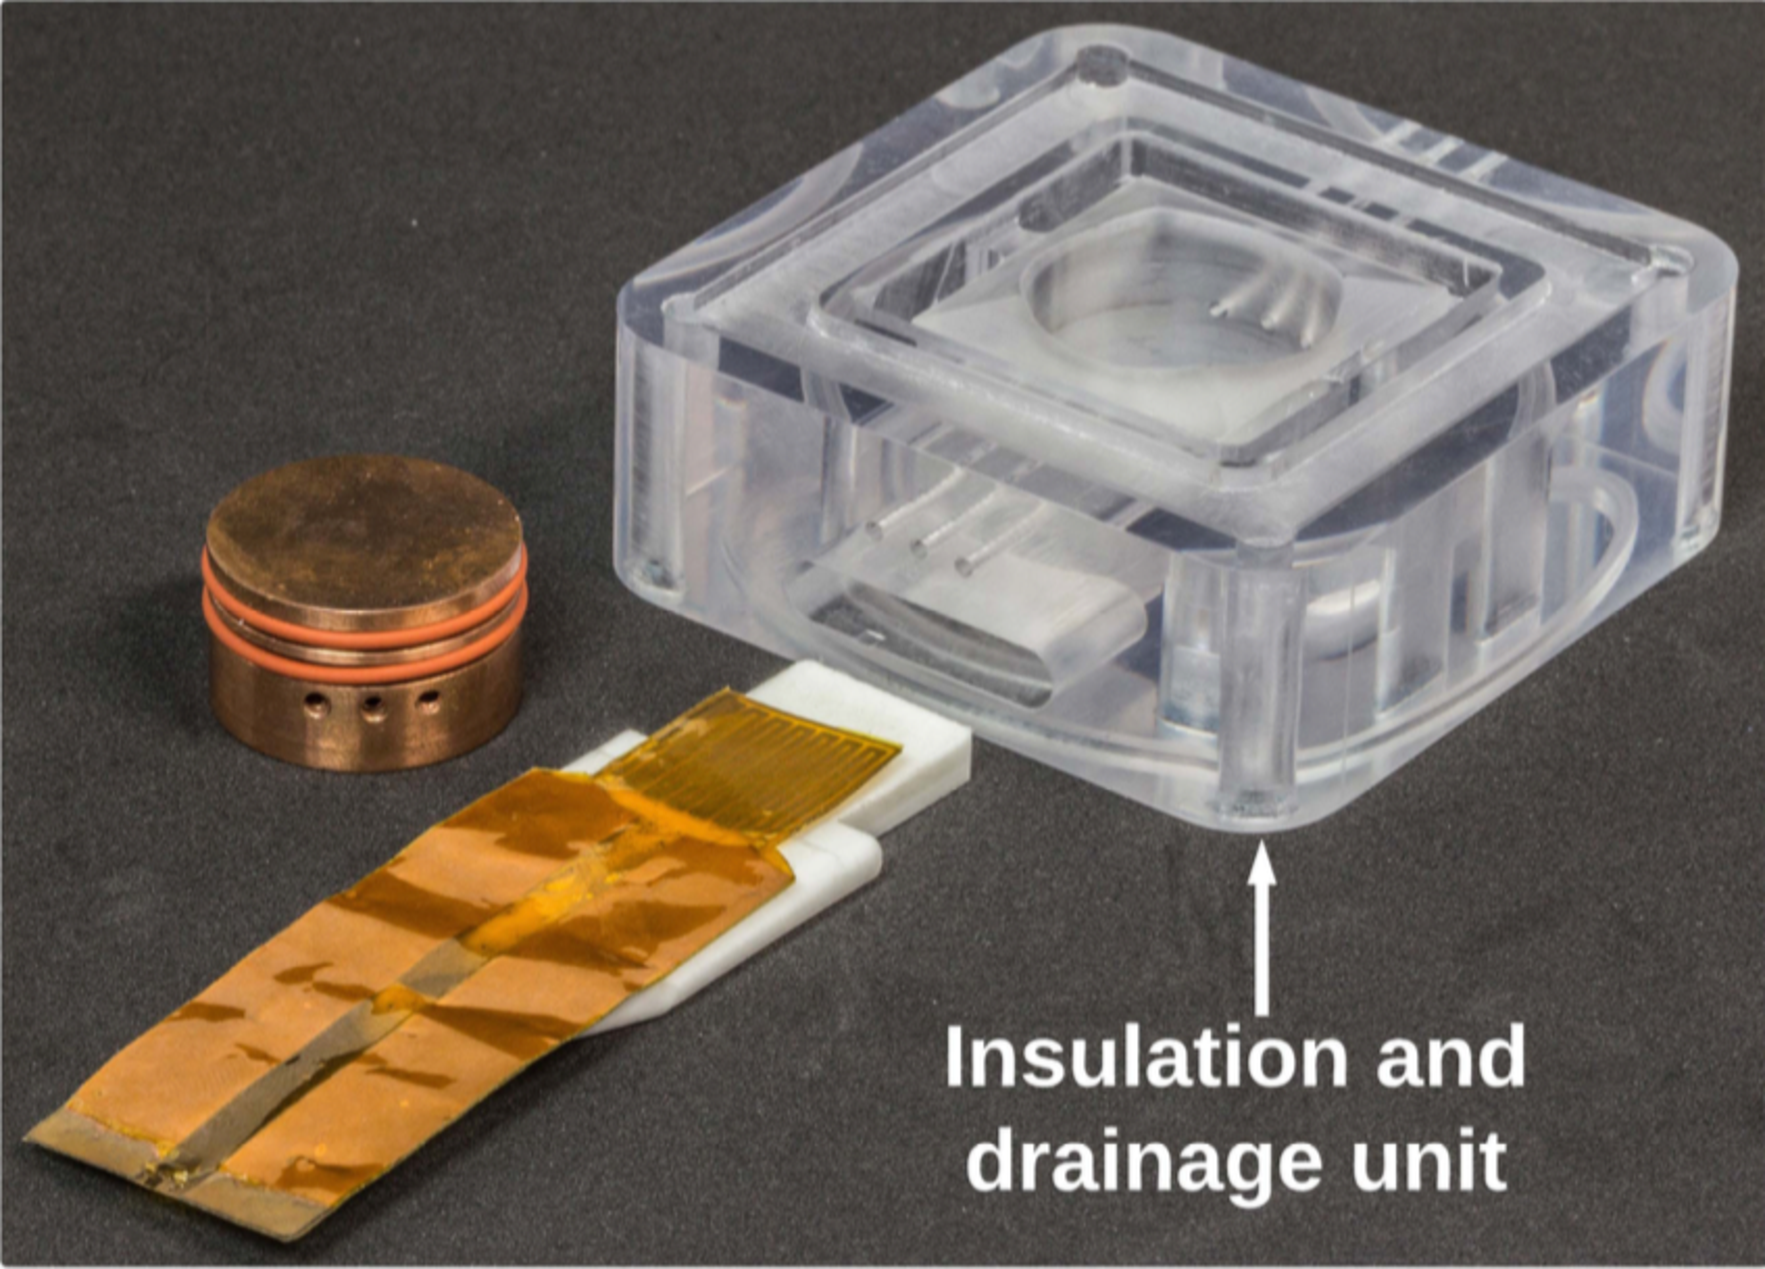
\includegraphics[height=2.0in]{Figure_5(a).pdf}}
\hfil
\subfigure[b][]{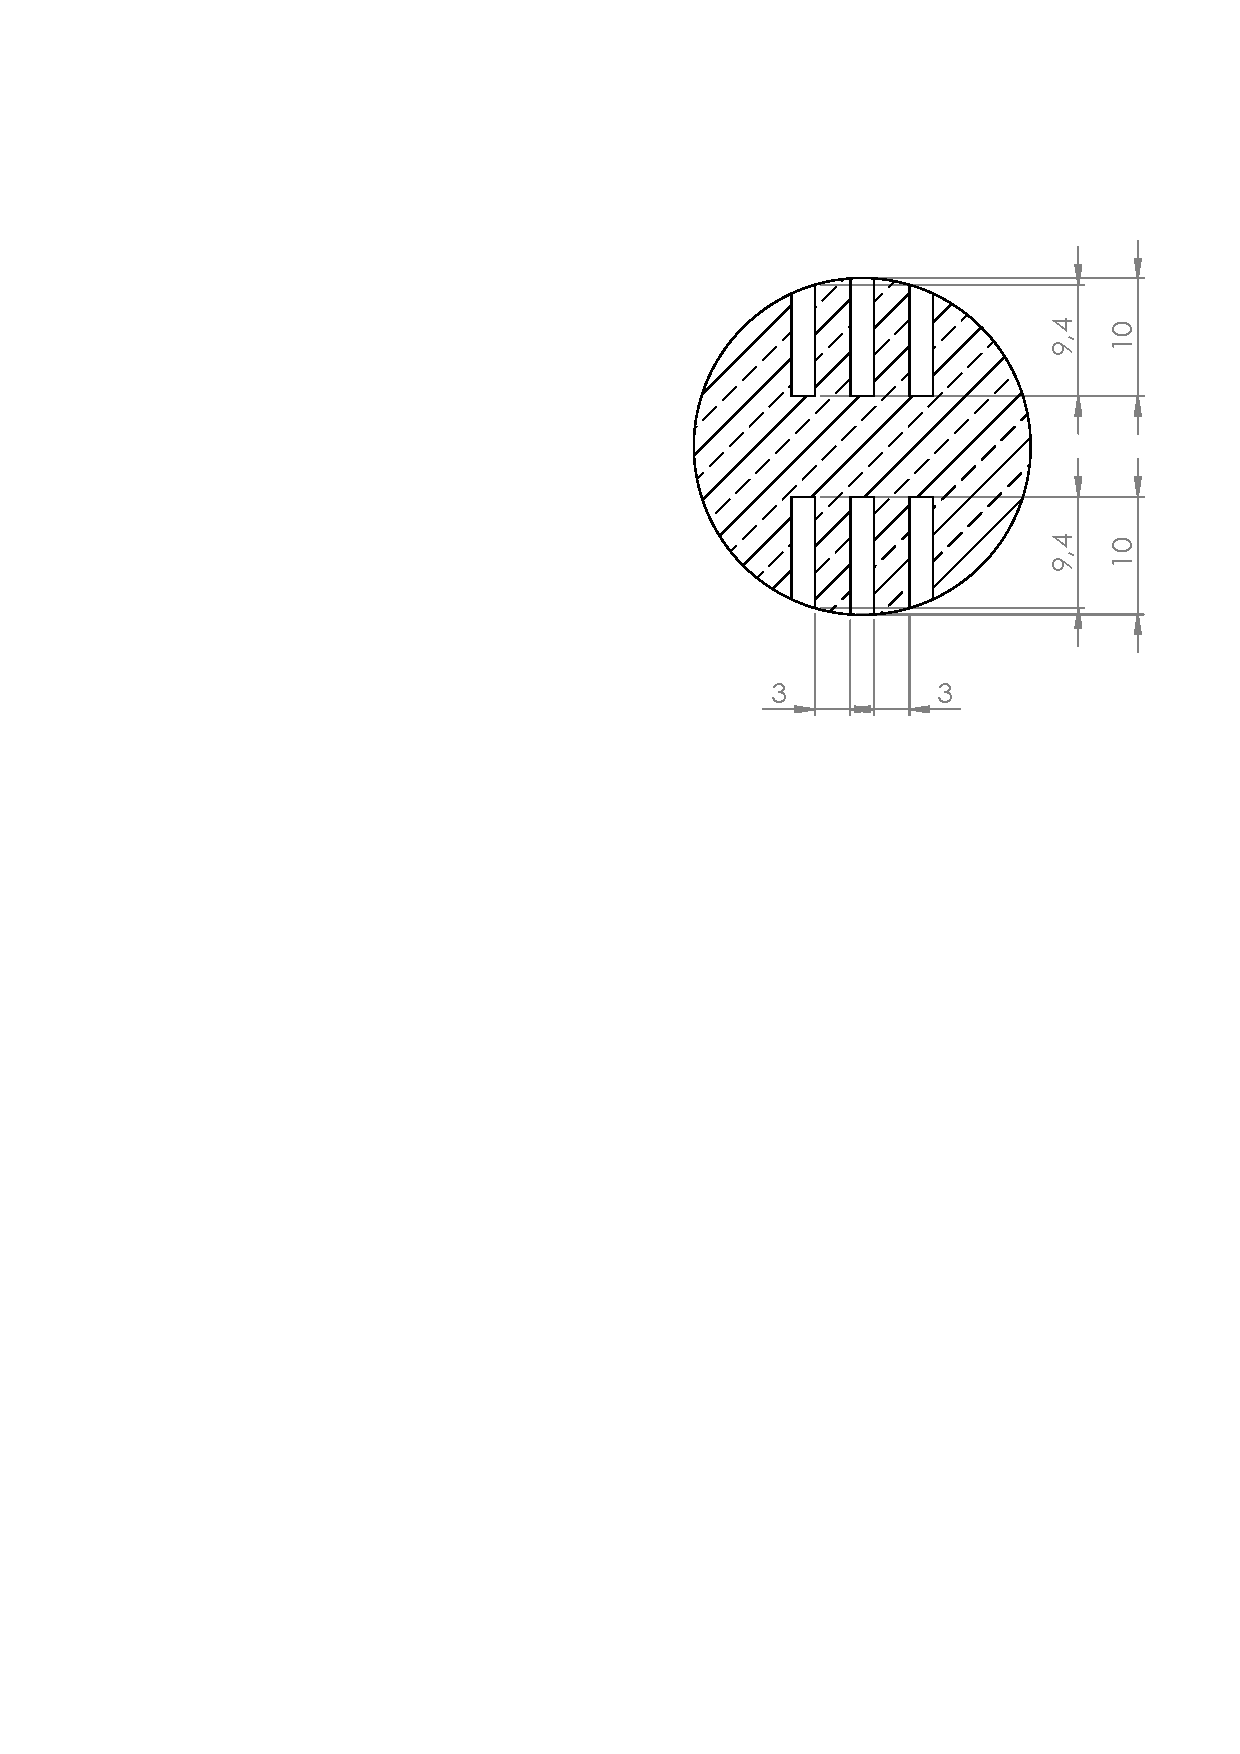
\includegraphics[height=2.0in]{Figure_5(b).pdf}}
\caption{(a) Bottom side components of the jet cooler (copper block, teflon base plate, film heater, and insulation and drainage unit). (b) Cross-section view of the copper block at the RTDs' plane (dimensions in millimeters).}
\label{fig:Figure_5}
\end{figure}
 
%A computer simulation using a commercial package (ANSYS Fluent 15) was carried out to determine the thermal losses in the insulation and drainage unit, i.e., the fraction of the input thermal load that actually reaches the top surface of the copper block (jet impinging surface). Accounting for the thermal losses help to correct the surface temperature and the jet impingement heat transfer coefficient. Thus, the correction factor for the input thermal load, $\kappa$, is defined as,

%\begin{equation}\label{Eq_1}
%\kappa = \Bigg| \frac{\dot{Q}_{c}^{*} - \dot{W}_{h}}{\dot{W}_{h}} \Bigg| \times 100\%
%\end{equation}

%\noindent where $\dot{Q}_{c}^{*}$ is the heat transfer rate effectively dissipated at the impingement surface and the input thermal load, $\dot{W}_{h}$, is given by the product of the voltage and the current provided by the DC power supply.

%The mathematical model accounted for different physical properties of the solid parts in the insulation and drainage unit, and considered the skin heater as a plane heat source with a prescribed heat flux equal to $\dot{W}_{h}/A_{h}$, where $A_{h}$ is the skin heater area (4 cm$^{2}$). More details about the numerical simulation (boundary conditions, number of mesh elements, numerical convergence) are presented in Ref.~\cite{Oliveira2016}. The value of $\dot{Q}_{c}^{*}$ was different for each experimental test because of its dependence on the experimental parameters, namely the input thermal load, the evaporating temperature, the mass flow rate (which influences the heat transfer coefficients used as boundary conditions on the surfaces covered by a flowing liquid film) and the impinging surface heat transfer coefficient itself. However, the simulations showed that the relative difference between $\dot{W}_{h}$ and $\dot{Q}_{c}^{*}$ was always smaller than 5\%. Therefore, in the data reduction, the thermal losses in the insulation and drainage unit were considered equal to 5\% of the input heat load ($\kappa$ = 5\%). 

%\nomenclature[Bkappa]{$\kappa$}{Correction factor for the cooling capacity [-]}%
\nomenclature[AQdot*c]{$\dot{Q}^{*}_{c}$}{Corrected cooling capacity [W]}%
%\nomenclature[AWdoth]{$\dot{W}_{h}$}{Input thermal load dissipated by the skin heater [W]}%
%\nomenclature[AAh]{$A_{h}$}{Skin heater area [m$^{\varA{2}}$]}%

\subsection{Experimental Conditions and Procedure}
\label{sec:Experimental_Conditions}

Experiments were conducted to investigate the influence of the following parameters on the system performance: (i) compressor piston displacement (stroke): 50\%, 75\% and 100\% of the full stroke; (ii) applied thermal load (cooling capacity): 25 to 160 W (the maximum cooling capacity achieved in a particular test); (iii) jet length: 28.84 and 9.75 mm, and (iv) hot reservoir (ambient) temperature: 15\textcelsius\ and 25\textcelsius. A 300-$\mu$m orifice diameter size was used in all test runs. The mass flow rate of the WEG mixture was kept fixed at 180 kg/h. The room temperature and the calorimeter temperature were set at 25\textcelsius. The compressor inlet superheat, defined as $\Delta T_{sh} = T_{1} - T_{evap}$, was kept fixed at 10\textcelsius\ (maximum expanded uncertainty of $\pm$ 0.31\textcelsius). 

\nomenclature[AH]{$H$}{Jet impingement length [mm]}%
\nomenclature[BDeltaTsh]{$\Delta T_{sh}$}{Refrigerant superheating degree [\textcelsius]}%

For a given piston stroke, $\alpha$, the applied thermal load was increased in steps until the critical heat flux (CHF) was reached, which explains the different number of tests for each condition. The CHF was characterized experimentally by a sudden increase of the heater surface temperature and was confirmed by visual observations to coincide with a partial or total dryout of the liquid film on the heater surface. 

\nomenclature[DCHF]{CHF}{Critical Heat Flux}%
\nomenclature[Balpha]{$\alpha$}{Compressor piston displacement (stroke) [\%]}%

The output (dependent) variables of the experimental apparatus are the refrigerant mass flow rate, pressures, temperatures, refrigerant sub-cooling degree at the outlet of the condenser, vapor mass quality at the outlet of the two-phase jet cooler, heat transfer rates and compressor power. Based on the output variables, the jet impingement heat transfer coefficient and the system coefficient of performance were calculated. 

All output data were recorded during a 15-minute interval, after guaranteeing that the variation of each experimental variable between the beginning and the end of that interval was less than two times the standard deviation associated with the measurements of that variable. Another criterion satisfied by each variable prior to data recording was the variable standard deviation over the 15-minute interval to be lower than or equal to the corresponding overall experimental uncertainty.

\subsection{Dependent Variables and Performance Metric}

Energy balances between the inlet and outlet of the condenser and superheating line (see Fig.~\ref{fig:Figure_1}) can be written as:

\begin{equation}\label{Eq_2}
\dot{Q}_{cond} = \dot{m}_{r} \left(h_{3} - h_{4}\right)	
\end{equation}
\begin{equation}\label{Eq_3}
\dot{Q}_{sh} = \dot{m}_{r} \left(h_{1} - h_{6}\right)	
\end{equation}

\nomenclature[AQdotcond]{$\dot{Q}_{cond}$}{Condenser heat transfer rate [W]}%
\nomenclature[AQdotsh]{$\dot{Q}_{sh}$}{Superheating heat transfer rate [W]}%
\nomenclature[Amdotr]{$\dot{m}_{r}$}{Refrigerant mass flow rate [kg h$^{\varA{-1}}$]}%
\nomenclature[Ah]{$h$}{Specific enthalpy [J kg$^{\varA{-1}}$]}%

\noindent where $\dot{m}_{r}$ is the refrigerant mass flow rate and the refrigerant enthalpy at the compressor inlet, $h_{1}$, condenser inlet, $h_{3}$, and condenser outlet, $h_{4}$, were computed via REFPROP 8.0 \cite{Lemmon2007} using the local experimental values of pressure and temperature. 

The refrigerant enthalpy at the outlet of the two-phase jet cooler, $h_{6}$, was calculated from the energy balance on the cooler, neglecting the kinetic and potential energy contributions. Thus:

\begin{equation}\label{Eq_4}
h_{6} = h_{5} + \frac{\dot{Q}_{c}}{\dot{m}_{r}}
\end{equation}

\nomenclature[AQdotc]{$\dot{Q}_{c}$}{Cooling capacity [W]}%

\noindent where $\dot{Q}_{c}$ is the cooling capacity and the refrigerant specific enthalpy at the inlet of the jet cooler, $h_{5}$, was also determined from local measurements of pressure and temperature  \textcolor{blue}{At steady state, the cooling capacity is equal to the thermal load imposed by the skin heater, considering a perfectly insulated test section}.

The vapor mass quality at the exit of the jet cooler, $x_{6}$, was determined from $h_{6}$ and the measured outlet pressure, $P_{6}$. The saturation pressures were calculated directly from the experimental data, i.e., $P_{evap} = P_{6}$ and $P_{cond} = P_{4}$, both taken at the outlets of the jet cooler and condenser, respectively.

\nomenclature[AP]{$P$}{Pressure [bar]}%
\nomenclature[Cevap]{$evap$}{Evaporating}%
\nomenclature[Ccond]{$cond$}{Condensing}%

The indicated power, i.e., the useful work performed on the refrigerant by the piston per unit time, can be determined by the following equation,

\begin{equation}\label{Eq_5}
\dot{W}_{ind} = \dot{m}_{r} \left(h_{2} - h_{1}\right)	
\end{equation}

\nomenclature[AWind]{$\dot{W}_{ind}$}{Indicated power [W]}%
\nomenclature[AWdotcomp]{$\dot{W}_{comp}$}{Electrical power consumption of the compressor [W]}%

\noindent where $h_{2}$ is the enthalpy at the compressor outlet computed using the local experimental values of pressure and temperature.% An energy balance on the compressor gives the energy rate dissipated as heat through the shell, $\dot{Q}_{shell}$, as the difference between the electrical power consumption, $\dot{W}_{comp}$, and the indicated power, $\dot{W}_{ind}$.

The jet impingement heat transfer coefficient, $\hbar$, is a key parameter in the design of the two-phase jet cooler. It is defined by: 

\begin{equation}\label{Eq_6}
\hbar = \frac{\dot{Q}_{c}^{*}}{A_{s} \left(T_{s} - T_{evap}\right)}
\end{equation}

\nomenclature[Ahbars]{$\hbar_{s}$}{Jet impingement heat transfer coefficient [W m$^{\varA{-2}}$ K$^{\varA{-1}}$]}% 
\nomenclature[AAs]{$A_{s}$}{Impingement surface area [cm$^{2}$]}%
\nomenclature[AT]{$T$}{Temperature [\textcelsius]}%
\nomenclature[ATs]{$T_{s}$}{Impingement surface temperature [\textcelsius]}%

\noindent where $A_{s}$ is the impingement surface area, $T_{evap}$ is the evaporating temperature and $\dot{Q}_{c}^{*}$ is the corrected cooling capacity, i.e., the fraction of the input heat load, $\dot{Q}_{c}$, that actually reaches the impingement surface \textcolor{blue}{of the copper block. The procedure to determine $\dot{Q}_{c}^{*}$ was outlined in detail in Ref.~\cite{OliveiraBarbosaJr.2016}, with the relative difference between $\dot{Q}_{c}^{*}$ and thermal load being of the order of 5\% for all tests.}% It was assumed that $\dot{W}_{h} = \dot{Q}_{c}$ for steady-state conditions and considering negligible thermal losses through the thermal insulation that covers the cooling system. 

The temperature of the surface of the copper block, $T_{s}$, was determined through a linear extrapolation of Fourier's law considering 1-D heat conduction in the axial direction,

\begin{equation}\label{Eq_7}
T_s = \overline{T}_{RTD} - \frac{L_s \dot{Q}_{c}^{*}}{k_{s} A_{s}}
\end{equation}

\nomenclature[ATRTDs]{$\overline{T}_{RTD}$}{Mean temperature of the RTDs in the copper block [\textcelsius]}%
\nomenclature[AL]{$L_{s}$}{Impingement surface-to-RTDs' plane distance [mm]}%
\nomenclature[Aks]{$k_{s}$}{Thermal conductivity of the heated surface [W m$^{\varA{-1}}$ K$^{\varA{-1}}$]}%

\noindent where $L_s$ is the distance between the copper block surface and the plane of the RTDs and $k_{s}$ is the thermal conductivity of copper evaluated at $\overline{T}_{RTD}$, which is the arithmetic mean of the five RTDs used to measure the copper block temperature.

In the present analysis, the coefficient of performance, $COP$, was defined so as to account for the energy consumption strictly necessary to remove the heat load imposed on the jet cooler. Thus:

\begin{equation}\label{Eq_8}
COP = \frac{\dot{Q}_{c}}{\dot{W}}
\end{equation}

\noindent where $\dot{W} = \dot{W}_{comp} + \dot{W}_{fan}$ is the sum of the power consumptions of the compressor and fan (recommended by the compressor manufacturer to cool the compressor shell). 

\nomenclature[ACOP]{$COP$}{Coefficient of performance [-]}%
\nomenclature[AWdot]{$\dot{W}$}{Total input power [W]}%
\nomenclature[AWdotfan]{$\dot{W}_{fan}$}{Electrical power consumption of a single cooler fan [W]}%



%\subsection{Calorimeter - Presentation and Working Principle}
%\label{sec:Calorimeter}
%
%A calorimeter was designed and built as a tool to indirectly determine the heat dissipation rate through the compressor shell and verify the closure of the system first-law energy balance. For that, the calorimeter needs to operate in a temperature-controlled environment and the temperature inside the calorimeter enclosure must be kept at a pre-determined value. Four external copper block-welded T-type thermocouples were positioned on each side of the enclosure and used to measure the room temperature, $T_{room}$, at the surroundings of the calorimeter. Analogously, five T-type thermocouples were used to determine the internal temperature of the enclosure, i.e., the calorimeter temperature, $T_{cal}$.
%
%The calorimeter is an enclosure (460 mm in length $\times$ 420 mm in width $\times$ 453 mm in height) manufactured from 20-mm thick low thermal conductivity (0.25 W m$^{\varA{-1}}$ K$^{\varA{-1}}$) acrylic plates, as depicted in Fig. \ref{fig:Figure_6}. A thermoelectric cooler (TEC) unit was mounted on the top wall of the calorimeter. The compressor and its inverter, four centrifugal fans (for temperature homogenization) and a 150-W tubular-finned air heater were assembled inside the calorimeter.
%
%\begin{figure}[!htp]
%\centering
%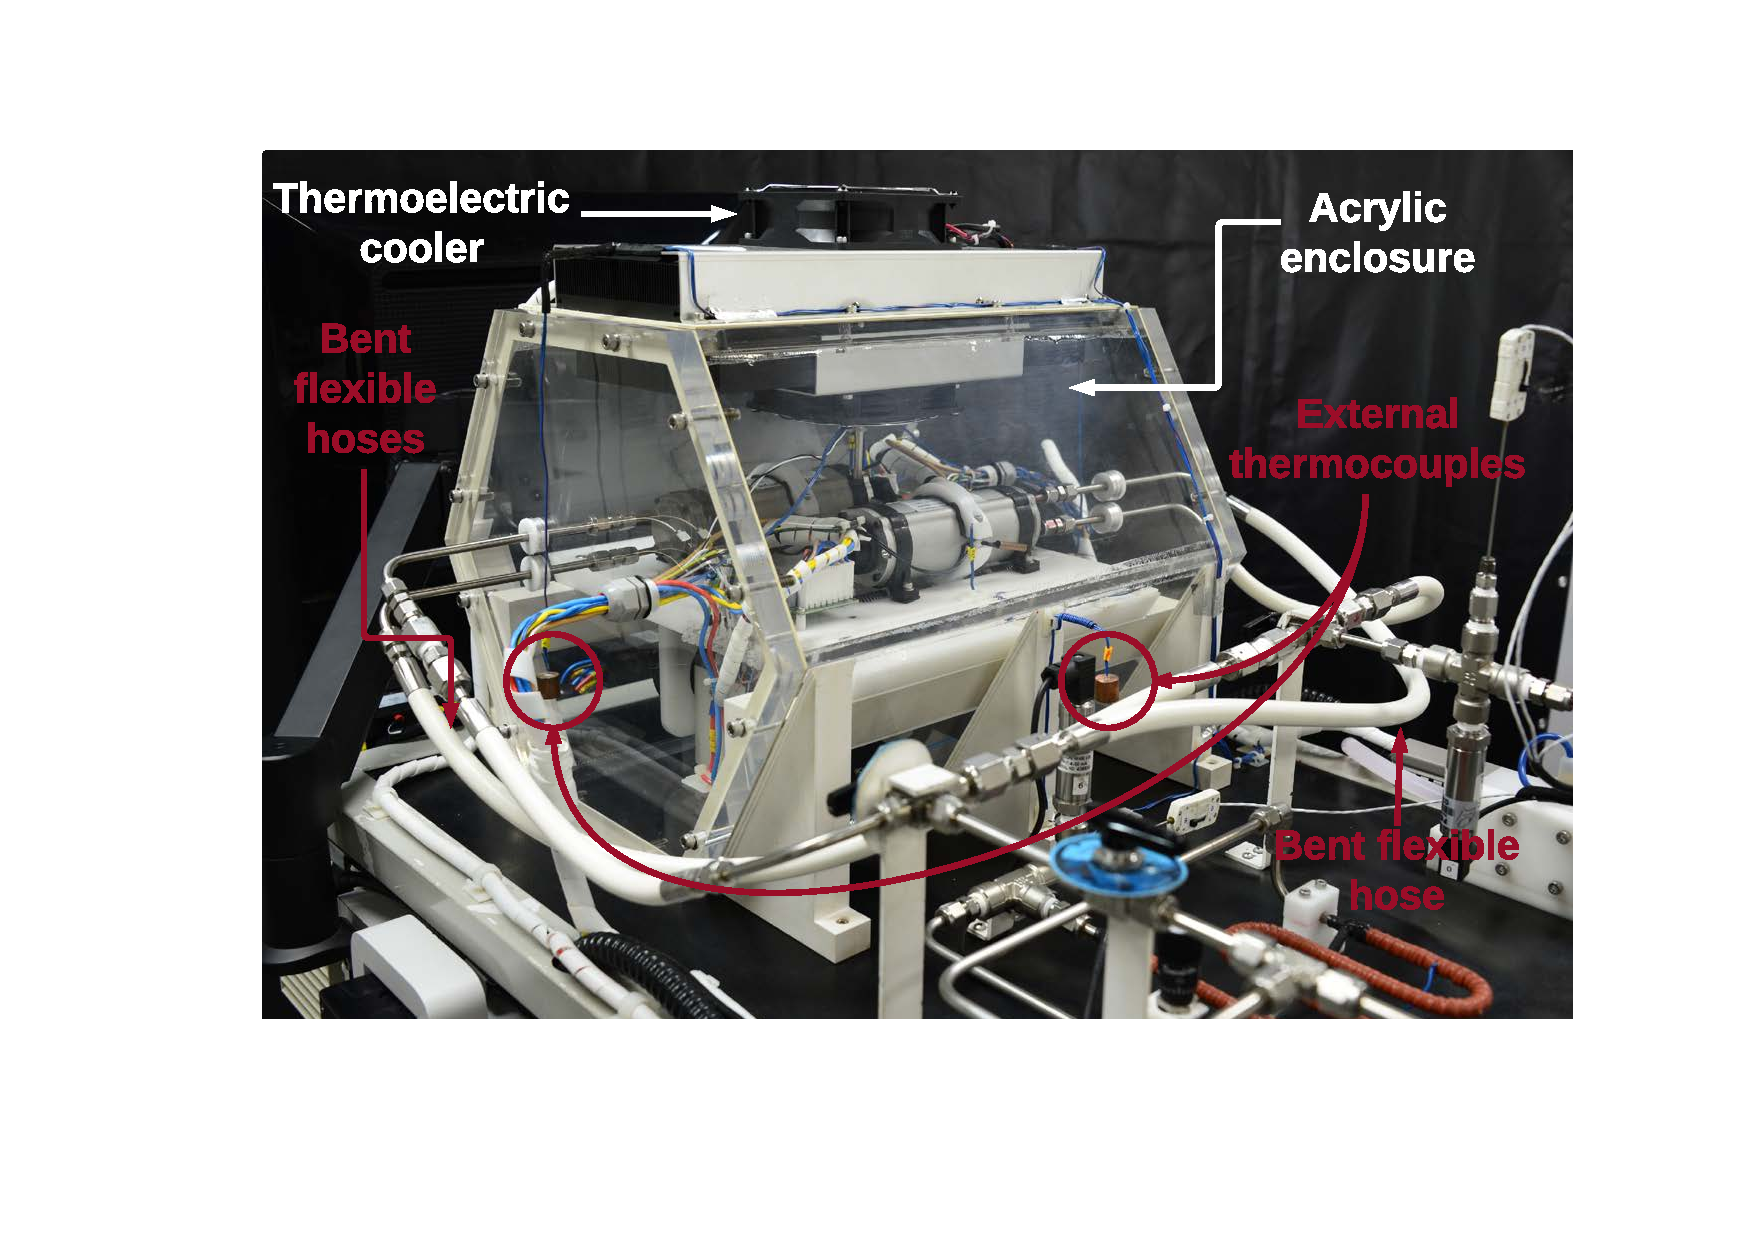
\includegraphics[angle=0,scale=0.45]{Figure_6.pdf}
%\caption{External view of the calorimeter.}
%\label{fig:Figure_6}
%\end{figure}
%
%The thermoelectric cooler was operated at the maximum cooling capacity, which corresponds to a calorimeter temperature difference $\Delta T_{cal} = |T_{room} - T_{cal}| = 0$. Considering this near-zero temperature difference and the very low thermal conductivity of the enclosure wall, it is reasonable to neglect the heat transfer rate through the walls. Thus, an energy balance was performed on the calorimeter considering all input and output heat transfer and work rates, according to Refs. \cite{OliveiraBarbosaJr.2016,Oliveira2016}, giving the expression for the calorimeter measurement of the heat dissipation rate through the compressor shell:
%
%\begin{equation}\label{Eq_9}
%\dot{Q}_{shell} = \dot{Q}_{TEC} - \dot{W}_{ah} - \dot{W}_{fans}
%\end{equation}

%\nomenclature[ATroom]{$T_{room}$}{Room temperature [\textcelsius]}%
%\nomenclature[ATcal]{$T_{cal}$}{Temperature inside the calorimeter [\textcelsius]}%
%\nomenclature[BDeltaTcal]{$\Delta T_{cal}$}{Calorimeter temperature difference [\textcelsius]}%
%\nomenclature[AQdotshell]{$\dot{Q}_{shell}$}{Heat transfer rate through the compressor shell [W]}%
%\nomenclature[AWdotah]{$\dot{W}_{ah}$}{Input thermal power dissipated by the air heater [W]}%
%\nomenclature[AWdotfans]{$\dot{W}_{fans}$}{Total electrical power consumption of the cooler fans [W]}%
%\nomenclature[AQdotTEC]{$\dot{Q}_{TEC}$}{Cooling capacity of the thermoelectric cooler [W]}%
%\nomenclature[Ccal]{$cal$}{Calorimeter heat balance}%
%\nomenclature[Ceb]{$eb$}{First-law energy (heat) balance}%
%\nomenclature[DTEC]{TEC}{Thermoelectric Cooler}%

%The cooling capacity of the thermoelectric cooler was experimentally determined for $\Delta T_{cal} =$ 0 (uncertainty of $\pm$ 0.10\textcelsius) at $T_{room}$ = $T_{cal}$ = 25\textcelsius\ (uncertainties of $\pm$ 0.09\textcelsius\ and $\pm$ 0.05\textcelsius, respectively) through a meticulous calibration procedure \cite{Oliveira2016}. According to the manufacturer, this is the operating temperature at which the maximum cooling capacity of the TEC occurs, i.e., $\dot{Q}_{TEC} = 143.42 \pm 4.23$ W. Additionally, the electrical power consumption of all fans, $\dot{W}_{fans}$, was obtained from a series of power measurements considering each centrifugal fan and the internal cooler fan of the TEC, i.e., $\dot{W}_{fans} = 57.33 \pm 3.10$ W. At each test run, the air heater thermal power, $\dot{W}_{ah}$, was measured using a power line transducer (uncertainty of $\pm$ 0.65 W).

\subsection{Energy balances and experimental uncertainties}

\textcolor{blue}{As discussed in Ref.~\cite{OliveiraBarbosaJr.2016},} energy balances were executed on the experimental apparatus for each experimental test to verify the consistency of the measurements. The first-law (\textcolor{blue}{energy} balance) residue, $\delta_{\rm 1st}$, is defined as the difference between the heat transfer rates out of and into the refrigeration system,

\begin{equation}\label{Eq_10}
\delta_{eb} = \frac{|\dot{Q}_{cond} - (\dot{Q}_{c} + \dot{Q}_{sh} + \dot{W}_{ind})|}{\dot{Q}_{c} + \dot{Q}_{sh} + \dot{W}_{ind}} \times 100\%
\end{equation}

\nomenclature[Bdelta]{$\delta$}{Energy balance residue [\%]}%

\textcolor{blue}{Additionally, a compressor calorimeter has been specially designed and constructed to provide a direct measure of the rate of heat dissipation by the compressor through its shell. A full description of the calorimeter is given in Refs.~\cite{OliveiraBarbosaJr.2016,Oliveira2016}}. %The calorimeter heat balance residue, $\delta_{cal}$, is defined as:

%\begin{equation}\label{Eq_11}
%\delta_{cal} = \frac{|\dot{Q}_{shell,cal} - \dot{Q}_{shell,eb}|}{\dot{Q}_{shell,eb}} \times 100\%
%\end{equation}
%
%\noindent where $\dot{Q}_{shell,cal}$ is computed from Eq.~\eqref{Eq_9} and $\dot{Q}_{shell,eb}$ is calculated from the energy balance on the compressor, i.e., $\dot{W}_{comp} - \dot{W}_{ind}$.

For the \textcolor{blue}{tests reported in this paper}, the average value of $\delta_{eb}$ was 0.9\%, which confirms that the \textcolor{blue}{energy} balance \textcolor{blue}{was} fully satisfied \textcolor{blue}{and that the experimental facility was properly insulated and the energy transfer rates were measured accurately. The compressor calorimeter energy balance was also satisfied (despite the somewhat larger average residue of 9.2\%), indicating that the energy transfer rates to and from the oil-free compressor were also measured accurately}.  

%The average value of $\delta_{cal}$ was higher, but still fairly small (9.2\%). This indicates that the experimental facility was properly insulated and the energy transfer rates were measured accurately. The maximum values of $\delta_{eb}$ and $\delta_{cal}$, which correspond to particularly challenging experimental runs, were 2.1\% and 14.8\%, respectively. 

Table~\ref{tab:Table_1} presents the expanded uncertainties for the calculated parameters, according to the procedure of Ref.~\cite{Coleman2009}. As these uncertainties vary according to each experimental run, only the maximum values are reported \cite{Oliveira2016}.

\begin{table}[!htbp]
	\caption{Expanded uncertainties (maximum values) of the calculated parameters.}   
	\label{tab:Table_1}
	\centering
	\normalsize
	\begin{tabular}{@{} cc @{}}
		\toprule
 		Calculated parameters & Expanded uncertainty\\\hline
		$\dot{Q}_{c}$ [W] & 1.77 \\
		$\dot{W}_{comp}$ [W] & 4.53\\
		$COP$ [-] & 0.49\\
		$x_{6}$ [-] & 0.013\\
		$\hbar_{s}$ [W m$^{-2}$ K$^{-1}$] & 433.0\\
		$T_{s}$ [\textcelsius] & 0.10\\
		$T_{cond}$ [\textcelsius] & 0.10\\
		$T_{evap}$ [\textcelsius] & 0.26\\
		$\Delta T_{sc}$ [\textcelsius] & 0.18\\\bottomrule
	\end{tabular}
\end{table}

\nomenclature[BDeltaTsc]{$\Delta T_{sc}$}{Refrigerant sub-cooling degree [\textcelsius]}%

\section{Results}

\subsection{Effect of the Orifice-to-Heater Distance (Jet Length)}

In this section, \textcolor{blue}{the results were generated for a hot source temperature fixed at $T_{7}$ = 15\textcelsius. For convenience,} the jet cooler parameters are evaluated first and the system performance is analyzed next. In order to provide a meaningful basis for comparing the results obtained with the two  \textcolor{blue}{jet lengths, $H$}, the same refrigerant mass flow rate was enforced \textcolor{blue}{in} the tests with a piston stroke of 50\% and cooling capacity of 25 W. This was achieved by adjusting the refrigerant mass (charge) in the system.

Considering similar operating conditions ($\alpha$ and $\dot{Q}_{c}$), Fig.~\ref{fig:Figure_7} (a) suggests that $T_{s}$ is insensitive to the change in the jet length. Nevertheless, it is important to observe \textcolor{blue}{in the same figure} that, for the intermediate and full stroke conditions, the reduction of $H$ shifted the point of dryout (CHF) to lower cooling capacities. \textcolor{blue}{This point corresponds to the highest cooling capacity for each curve and, as mentioned above, is associated with a drastic increase of the heater surface temperature, resulting in the interruption of the experiment. As can be seen, the reduction of the CHF} was very dramatic, with a maximum \textcolor{blue}{decrease} of approximately 85 W for the 100\% piston stroke in comparison with the tests with a  \textcolor{blue}{larger $H$}. A clear reduction of the heat transfer coefficient was also observed when $H$ \textcolor{blue}{was} shortened from 28.84 to 9.75 mm, as seen in Fig.~\ref{fig:Figure_7} (b).

The behavior of the evaporating temperature is shown in Fig.~\ref{fig:Figure_8}. While the results for the two values of  \textcolor{blue}{$H$} are very similar for $\alpha =$ 50\%, the evaporating temperature for smaller jet lengths is reduced as the cooling capacity increases for $\alpha =$ 75\% and 100\%. %\textcolor{blue}{The reduction of evaporating pressure can be explained by the higher two-phase flow pressure drop in the superheating line, which, as will be seen, was caused by the higher liquid content at the outlet of the test section.} 
Thus, the net effect of the results shown in Figs.~\ref{fig:Figure_7} and \ref{fig:Figure_8} is an increase of the wall superheat, ($T_{s} - T_{evap}$), as  \textcolor{blue}{$H$} is reduced from 28.84 mm to 9.75 mm. 




%\newpage

\begin{figure}[!htp]
\centering
\subfigure[a][]{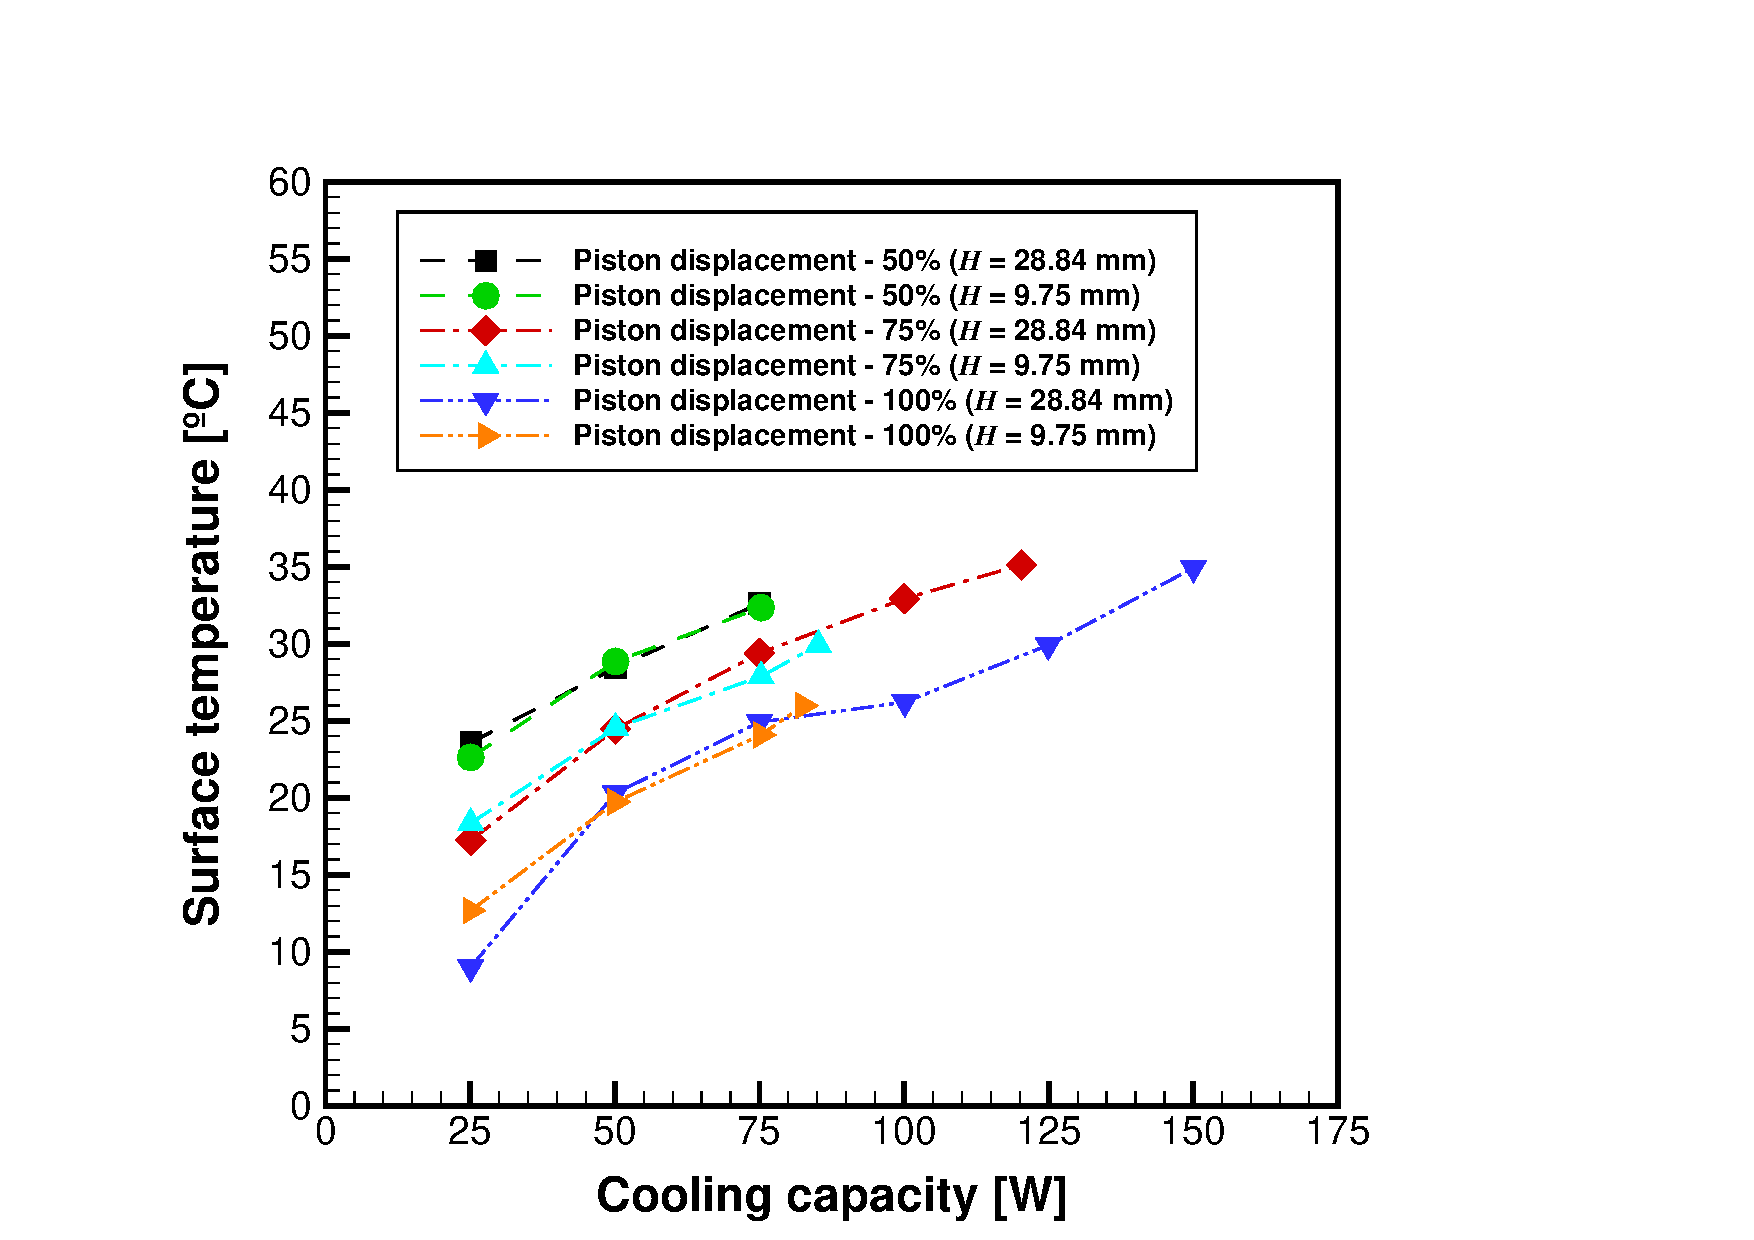
\includegraphics[angle=0,scale=0.325]{Figure_7(a).pdf}}
\hfil
\subfigure[b][]{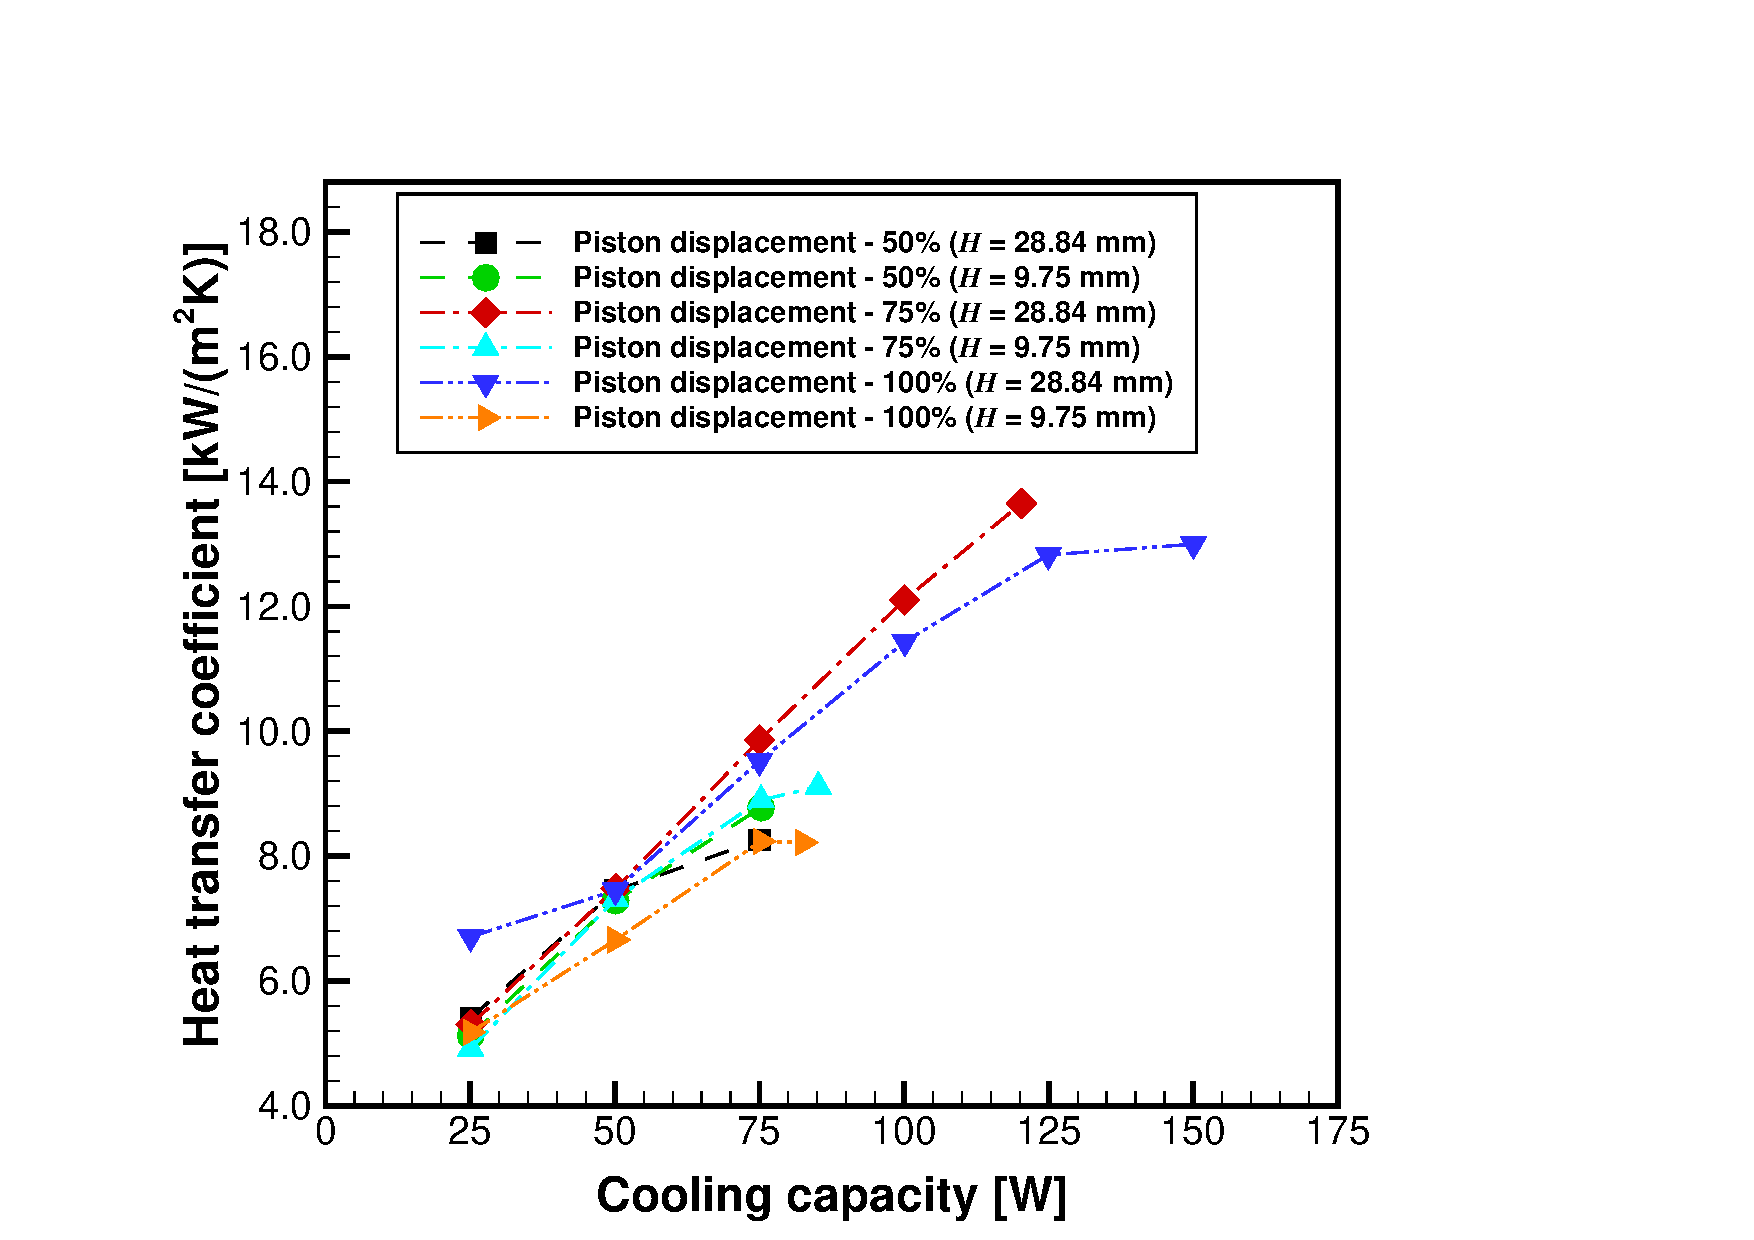
\includegraphics[angle=0,scale=0.325]{Figure_7(b).pdf}}
\caption{Jet cooler heat transfer parameters as a function of the applied heat load (cooling capacity) for different piston strokes and jet lengths. (a) Surface temperature. (b) Heat transfer coefficient. \colorbox{yellow}{Formato unidades HTC IJR na fig b}}
\label{fig:Figure_7}
\end{figure}

\begin{figure}[!htp]
\centering
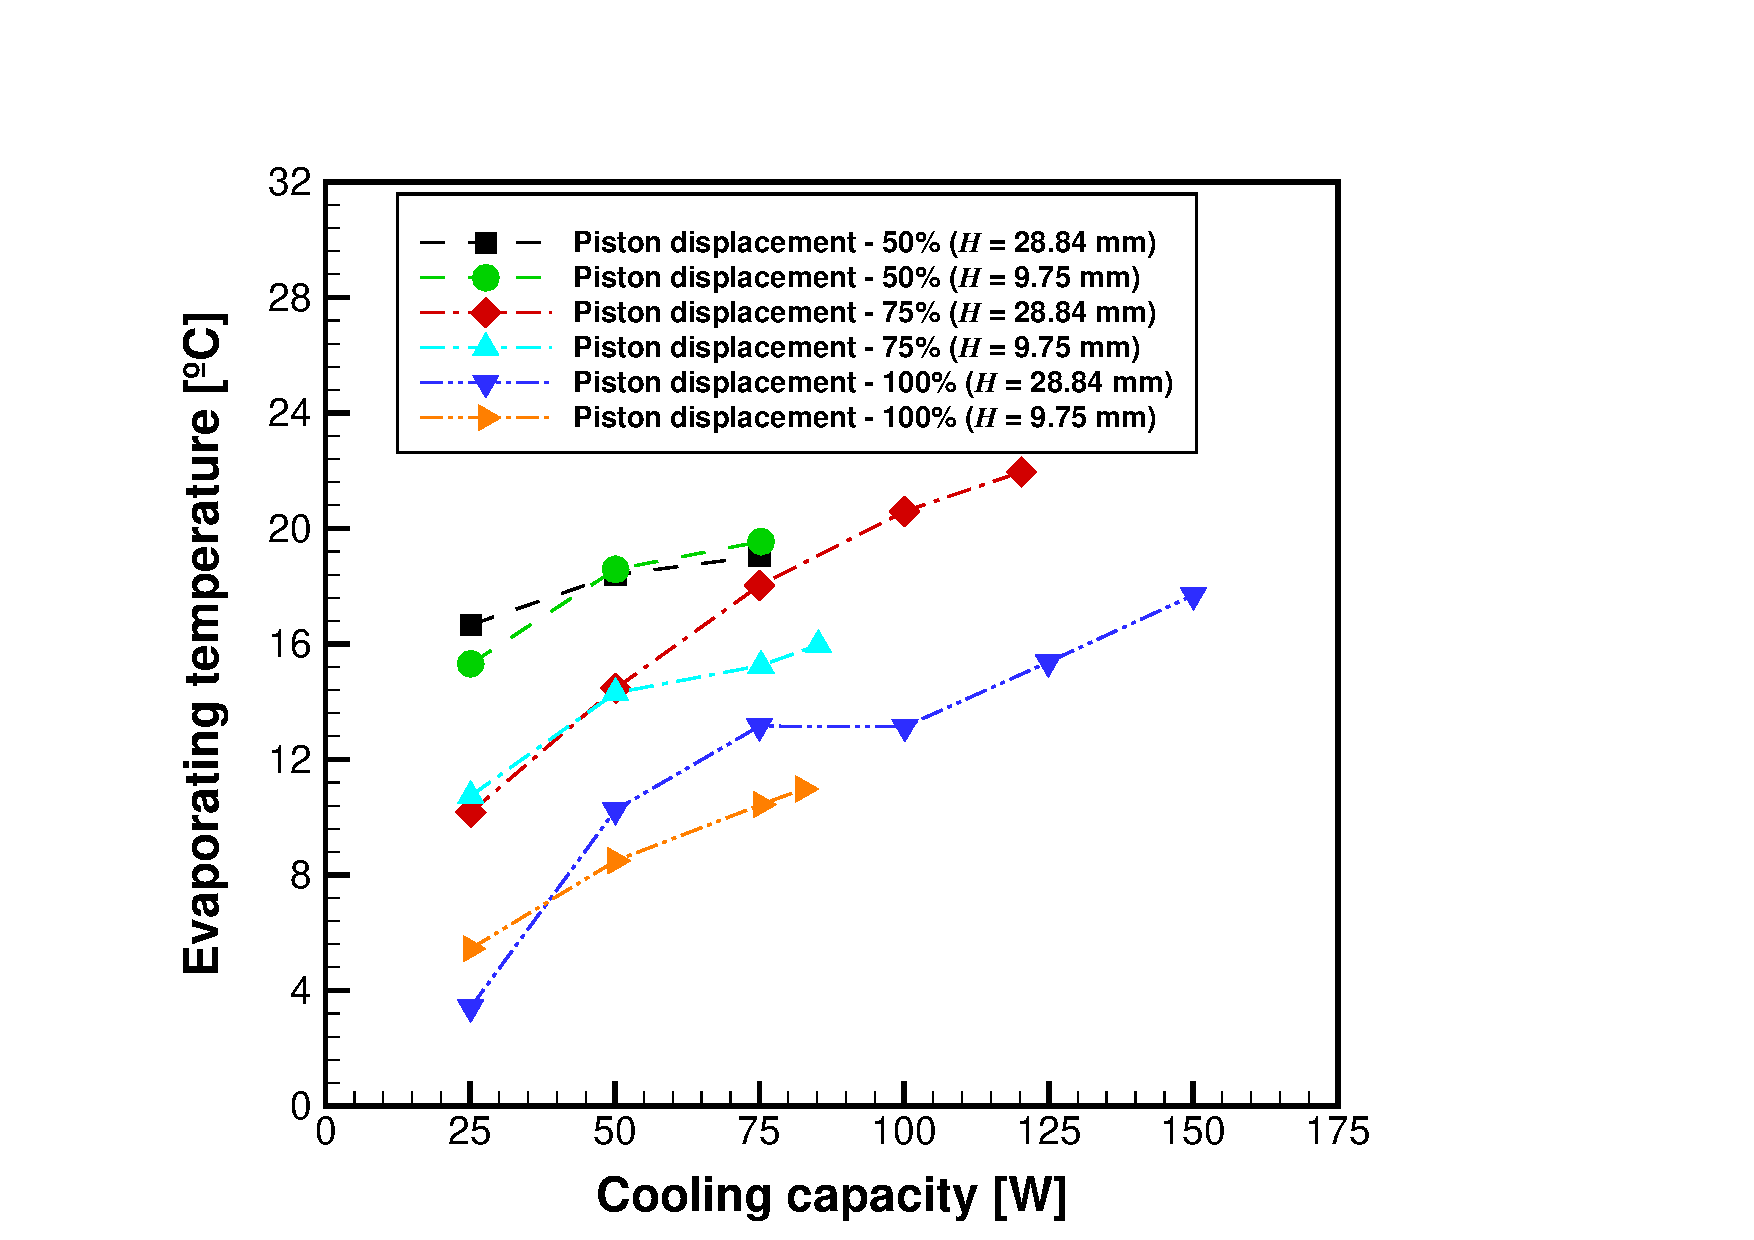
\includegraphics[angle=0,scale=0.375]{Figure_8.pdf}
\caption{Evaporating temperature as a function of the applied heat load (cooling capacity) for different piston strokes and jet lengths.}
\label{fig:Figure_8}
\end{figure}

For a fixed thermal load, \textcolor{blue}{it became clear that} the increase in wall superheat \textcolor{blue}{was} caused by a reduction of the \textcolor{blue}{thermal conductance associated with} the jet impingement  \textcolor{blue}{configuration}. Jet splattering and droplet breakup were the major factors contributing to the reduction of the heat transfer coefficient shown in Fig.~\ref{fig:Figure_7} (b). Splattering was visually observed to increase considerably when the  \textcolor{blue}{jet} length was reduced from 28.84 to 9.75 mm.  \textcolor{blue}{Since} the pressure ratio and the refrigerant mass flow rate were quite similar for the two values of $H$, the jet impact velocity is expected to be greater for the shorter jet length, which is likely to promote a more vigorous atomization of the liquid into droplets ejected from the heater surface. By having a lower flow rate of liquid as a continuous film on the surface, \textcolor{blue}{both} the heat transfer coefficient \textcolor{blue}{and the CHF} associated with the smaller $H$ \textcolor{blue}{are} reduced in comparison with the \textcolor{blue}{larger jet length}. 

\begin{figure}[!htp]
\centering
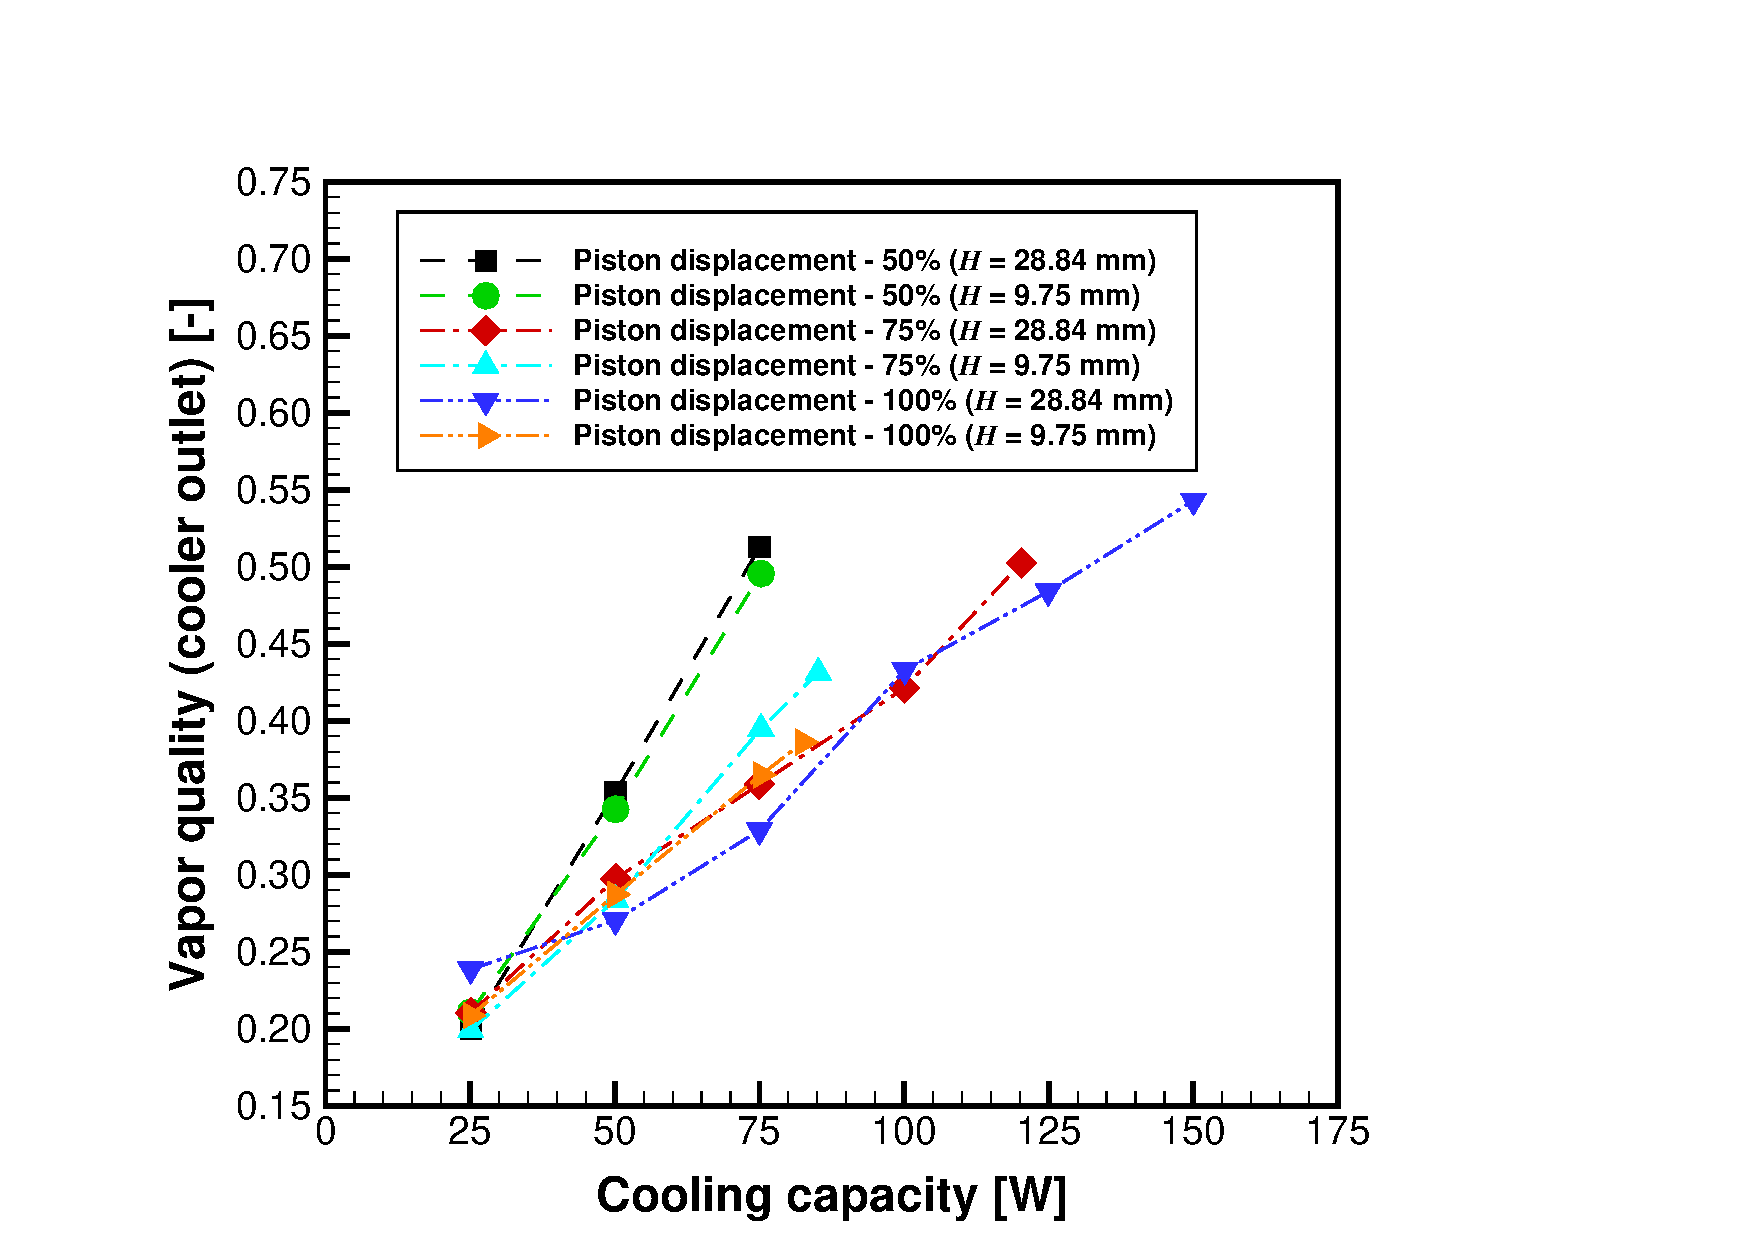
\includegraphics[angle=0,scale=0.375]{Figure_9.pdf}
\caption{Outlet vapor quality as a function of the applied heat load (cooling capacity) for different piston strokes and jet lengths.}
\label{fig:Figure_9}
\end{figure}

From an operation standpoint, the reduction of the  \textcolor{blue}{CHF appears to be} more important than the deterioration of the heat transfer coefficient. The effect of this reduction can also be perceived by looking at the behavior of the outlet vapor quality presented in Fig.~\ref{fig:Figure_9}. While the highest vapor qualities for the smaller jet length (considering piston strokes of 75\% and 100\%) are approximately 43\% and 39\%, the corresponding values for the longer jet are 50\% and 54\%, respectively, which means that the latent heat (enthalpy) of vaporization of the refrigerant is used much more effectively for a jet length of 28.84 mm. 

Figure \ref{fig:Figure_10} illustrates the effect of the jet length on the  \textcolor{blue}{thermodynamic} cycle for $\alpha = 100\%$ and $\dot{Q}_{c} = 75$ W. A clear shift towards lower condensing and evaporating pressures is observed due to the reduction of the pressure lift. 

\begin{figure}[!htp]
\centering
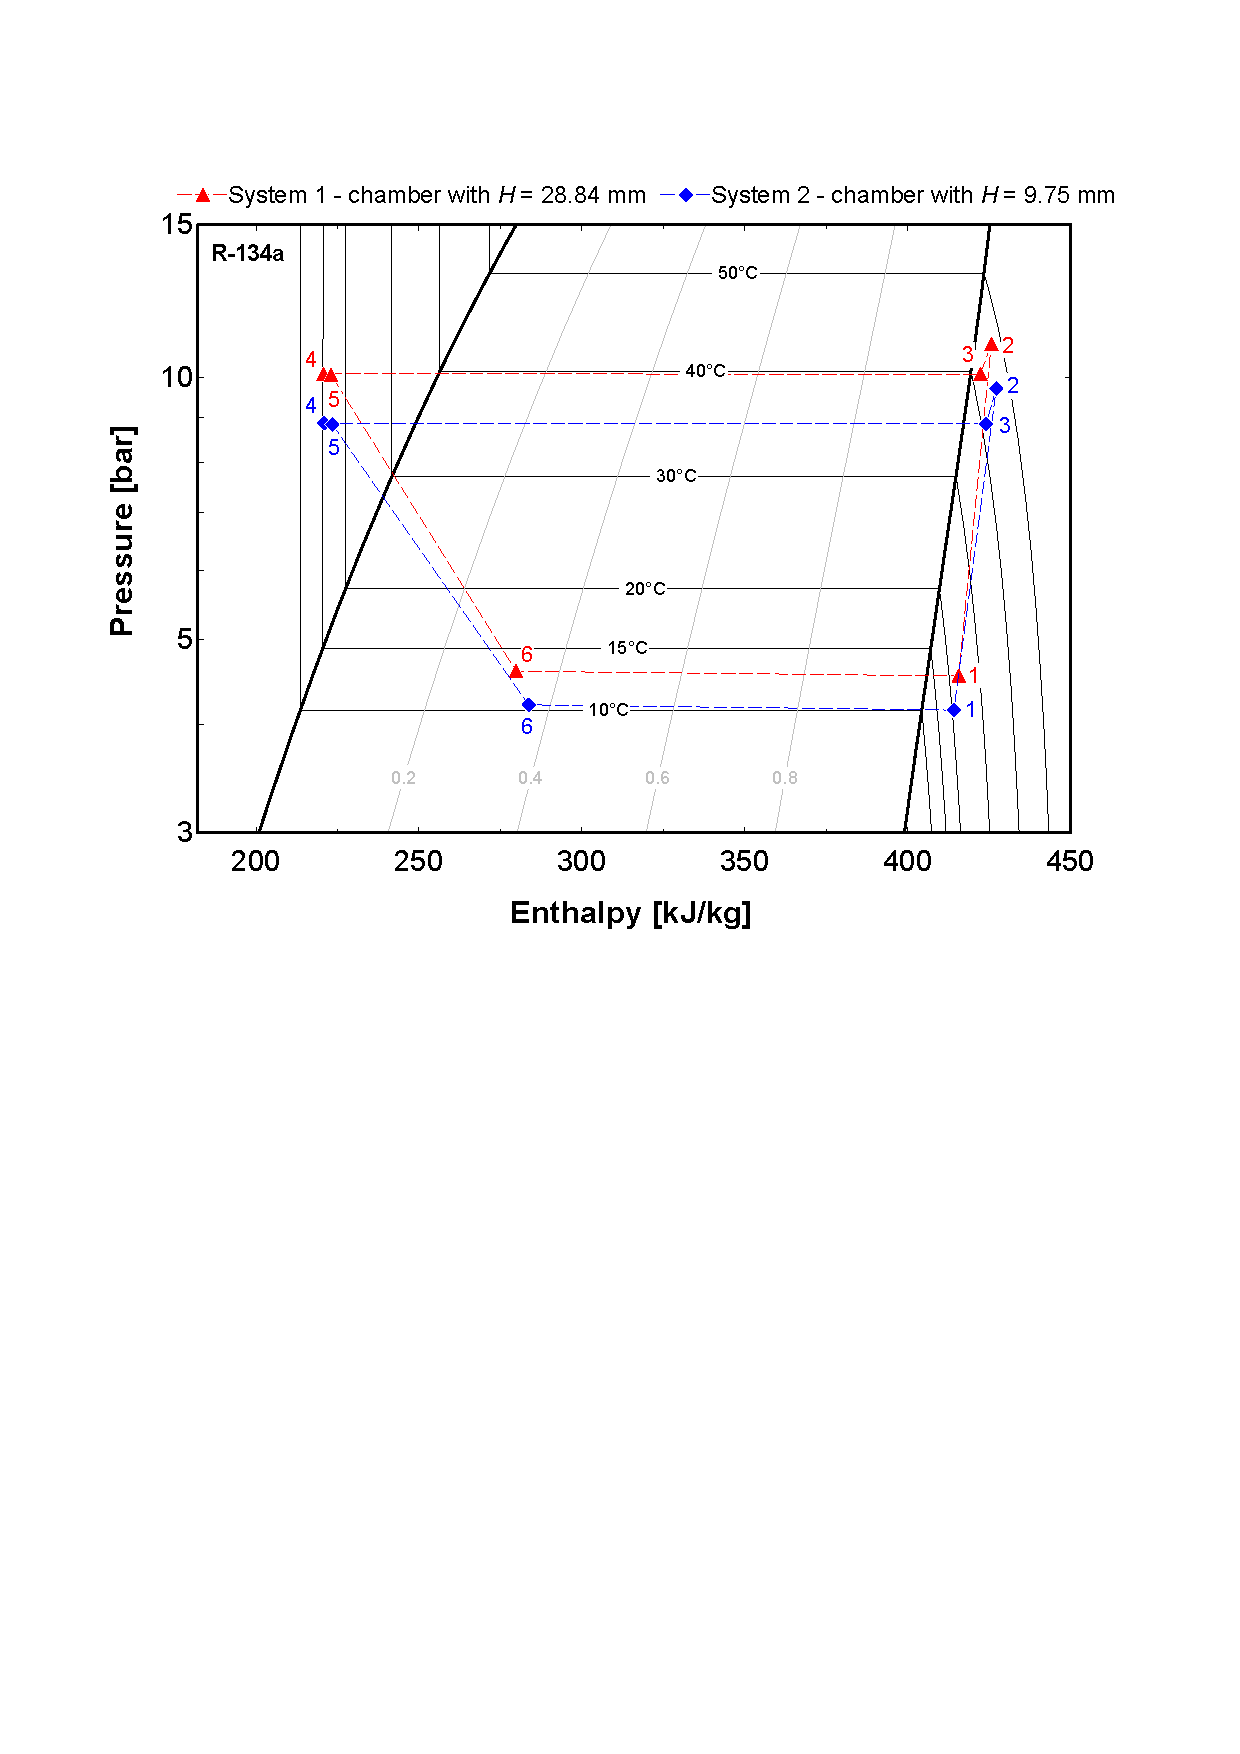
\includegraphics[angle=0,scale=0.6]{Figure_10.pdf}
\caption{$P$-$h$ diagram: comparison between different jet lengths for the same piston stroke (100\%) and cooling capacity (75 W). The numbers refer to the diagram in Fig.~\ref{fig:Figure_1}. \colorbox{yellow}{unidade formato  IJR eixo x}}
\label{fig:Figure_10}
\end{figure} 

Nevertheless, the effect of \textcolor{blue}{the above-mentioned} pressure shift on the compressor power consumption is rather small, as seen in Fig. \ref{fig:Figure_11} (a). Therefore, the $COP$ is mildly affected, i.e., there is only a slight increase for piston strokes of 75\% and 100\%, as depicted in Fig. \ref{fig:Figure_11} (b).

\begin{figure}[!htp]
\centering
\subfigure[a][]{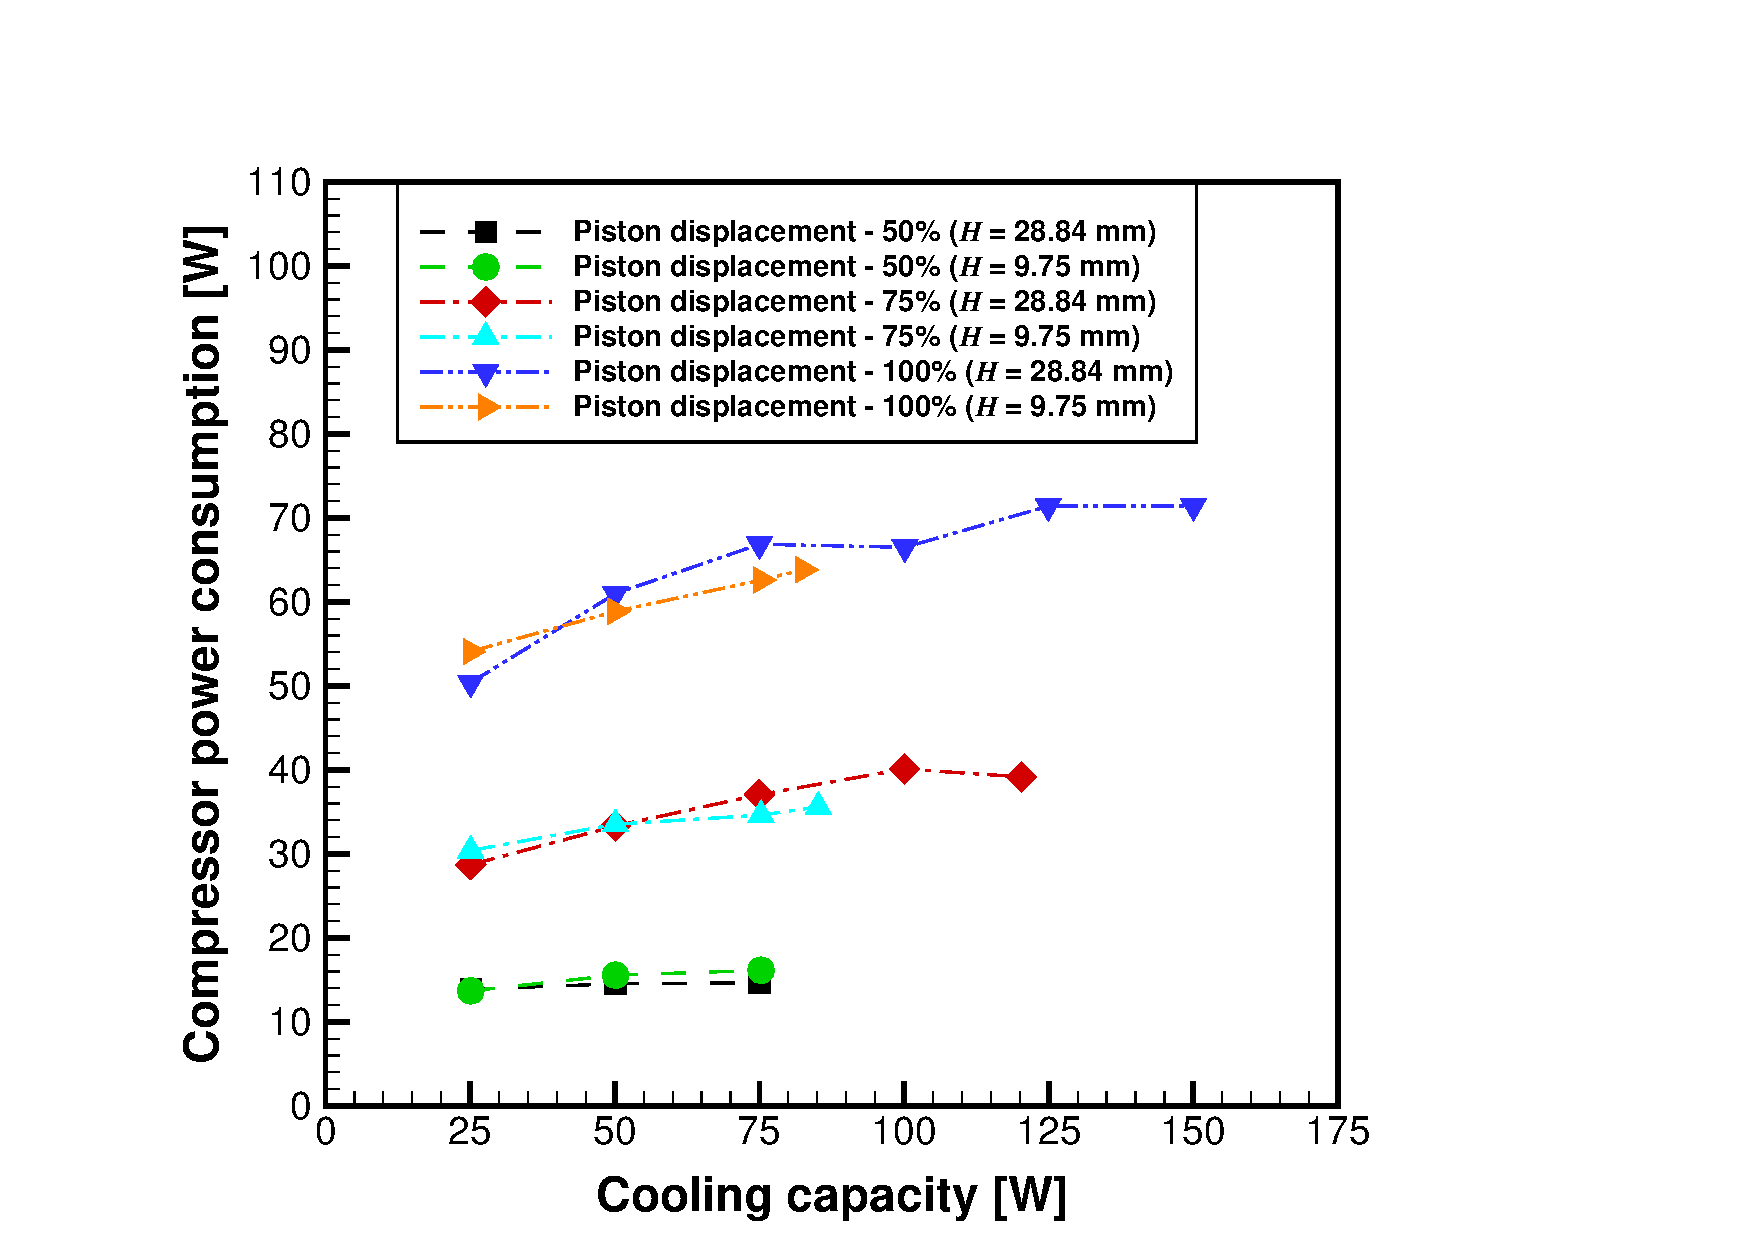
\includegraphics[angle=0,scale=0.325]{Figure_11(a).pdf}}
\hfil
\subfigure[b][]{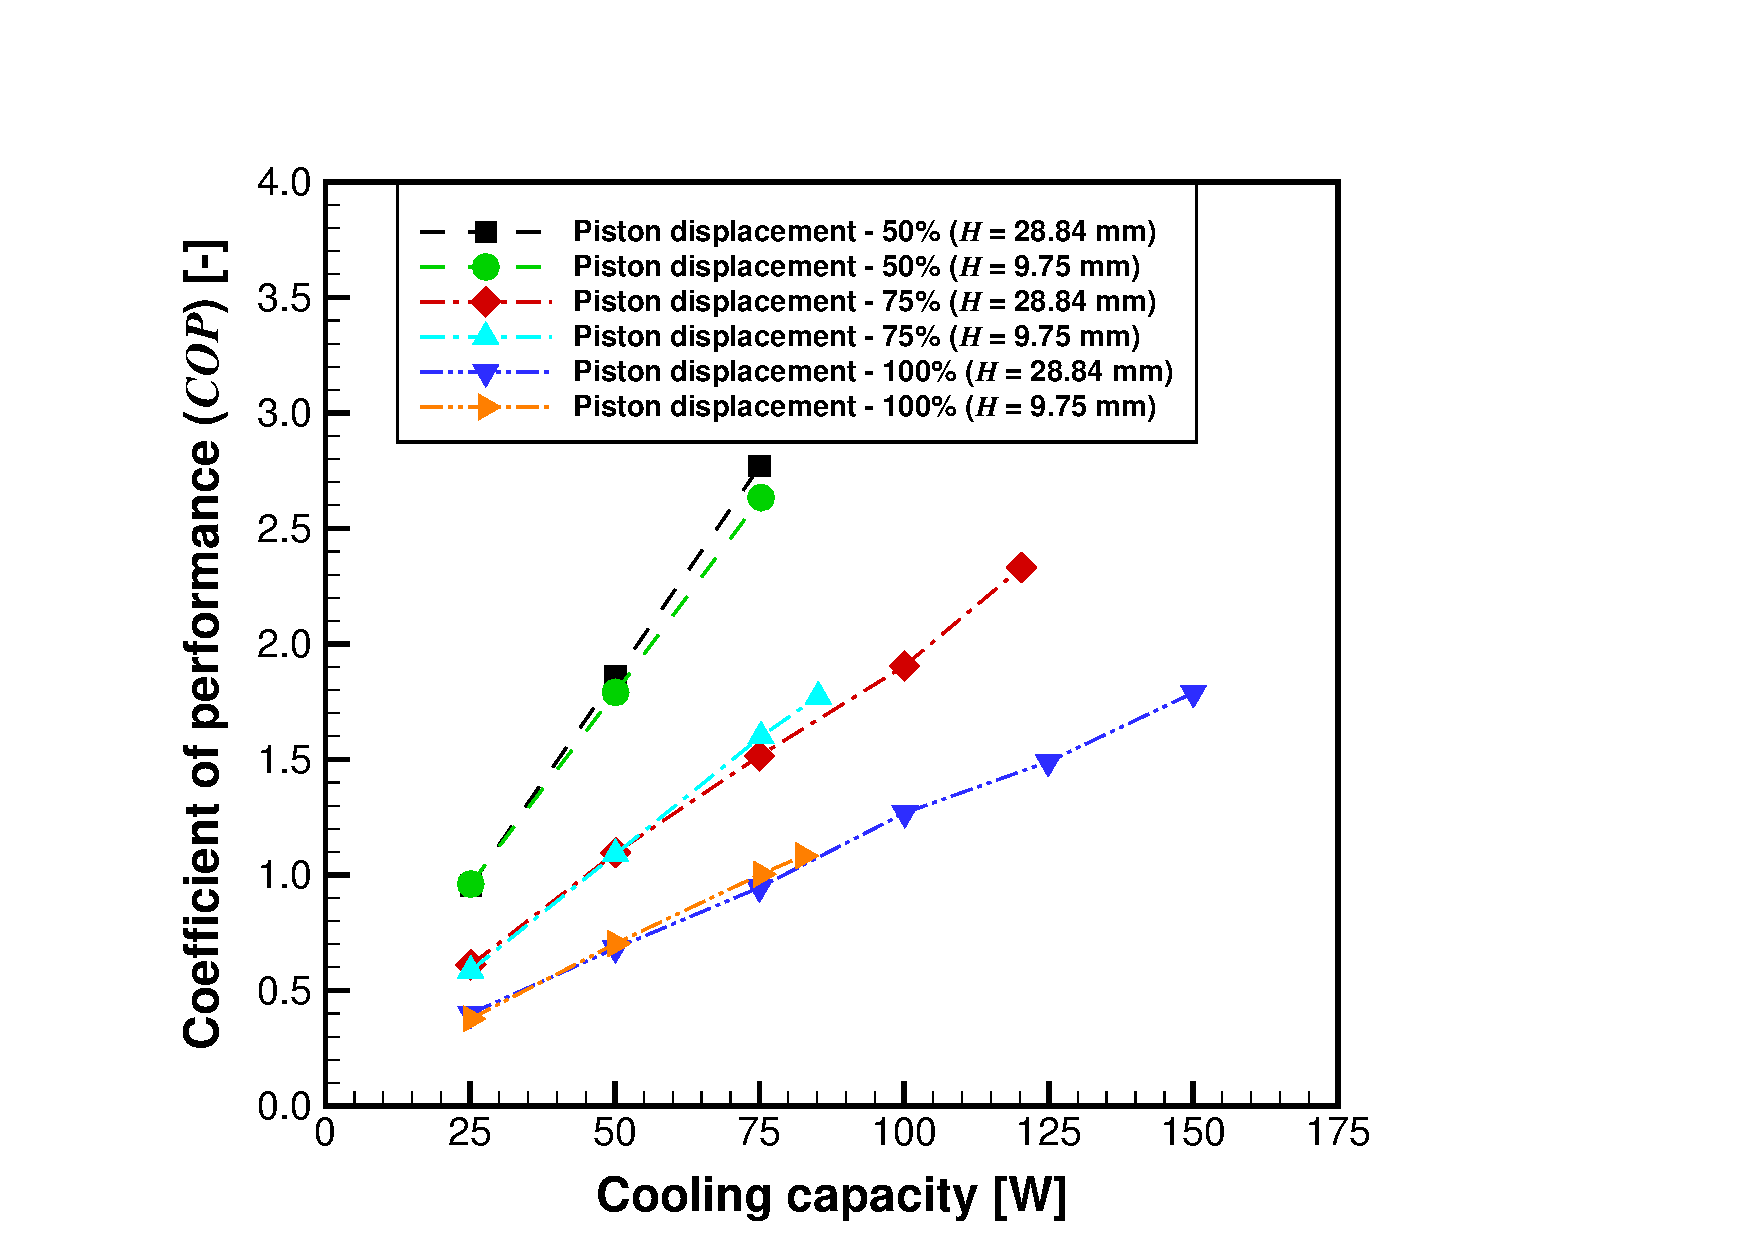
\includegraphics[angle=0,scale=0.325]{Figure_11(b).pdf}}
\caption{(a) Compressor power consumption and (b) $COP$ as a function of the applied heat load (cooling capacity) for different piston strokes and jet lengths.}
\label{fig:Figure_11}
\end{figure}

\subsection{Effect of the Hot Reservoir (Ambient) Temperature}


This section is dedicated to the analysis of the effect of the hot \textcolor{blue}{end} (secondary fluid) temperature, $T_{7}$. The experimental tests were run only at 100\% compressor stroke, \textcolor{blue}{for it has been shown \cite{OliveiraBarbosaJr.2016,Oliveira2016}} that it is more \textcolor{blue}{(thermodynamically)} advantageous to operate the active cooling system at such conditions.

Operating the system at a higher hot end temperature (HET) increases the condensing temperature compared to the cases for which $T_{7}$ = 15\textcelsius, as \textcolor{blue}{shown} in Fig.~\ref{fig:Figure_12} (a). In addition, a higher hot end temperature necessarily increases the refrigerant temperature at the condenser outlet, $T_{4}$. As the rise in $T_{7}$ is significantly higher than the increase in $T_{4}$ for both hot end temperatures, the sub-cooling degree, defined as $\Delta T_{sc} = T_{cond} - T_{4}$, decreases as exhibited in Fig.~\ref{fig:Figure_12} (b). Therefore, the coolant reaches the jet heat sink at a higher temperature. 

\begin{figure}[!htp]
\centering
\subfigure[a][]{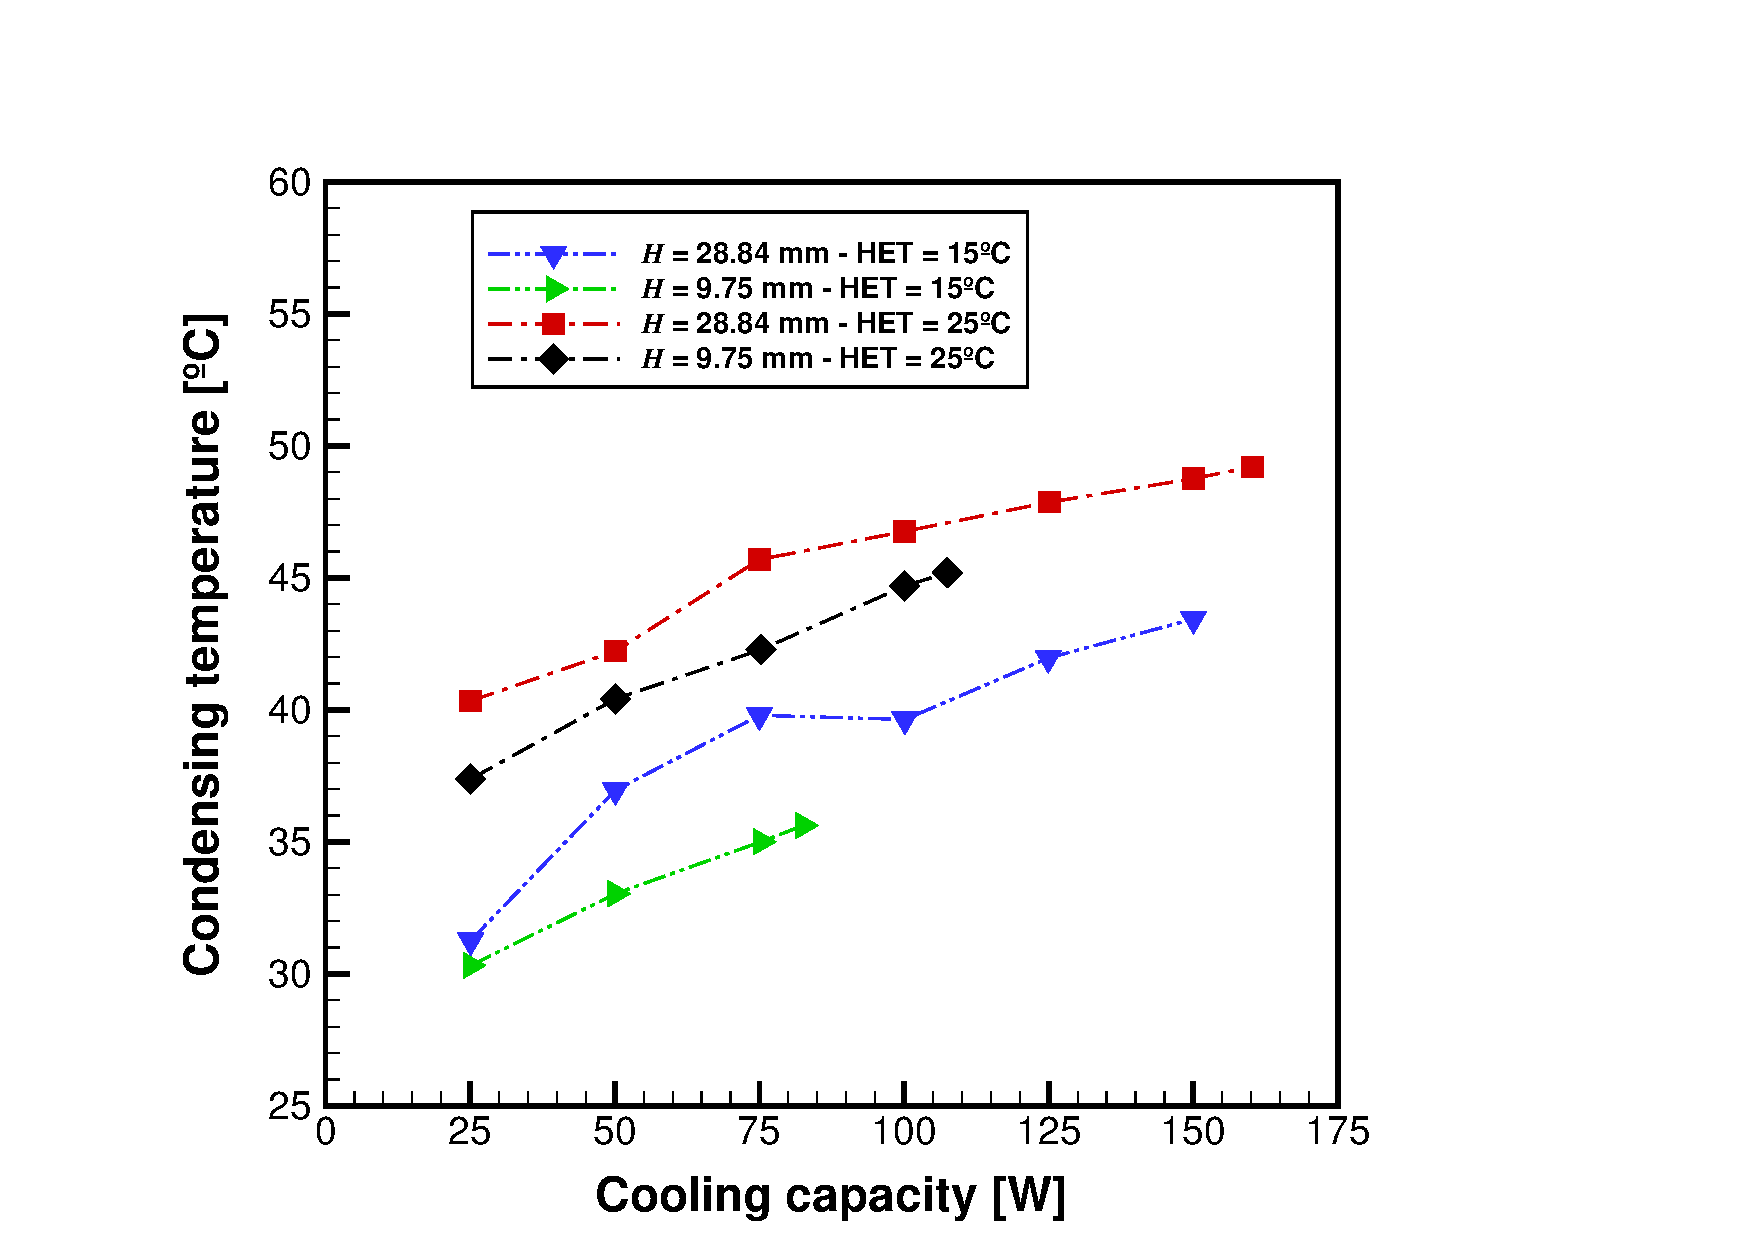
\includegraphics[angle=0,scale=0.325]{Figure_12(a).pdf}}
\hfil
\subfigure[b][]{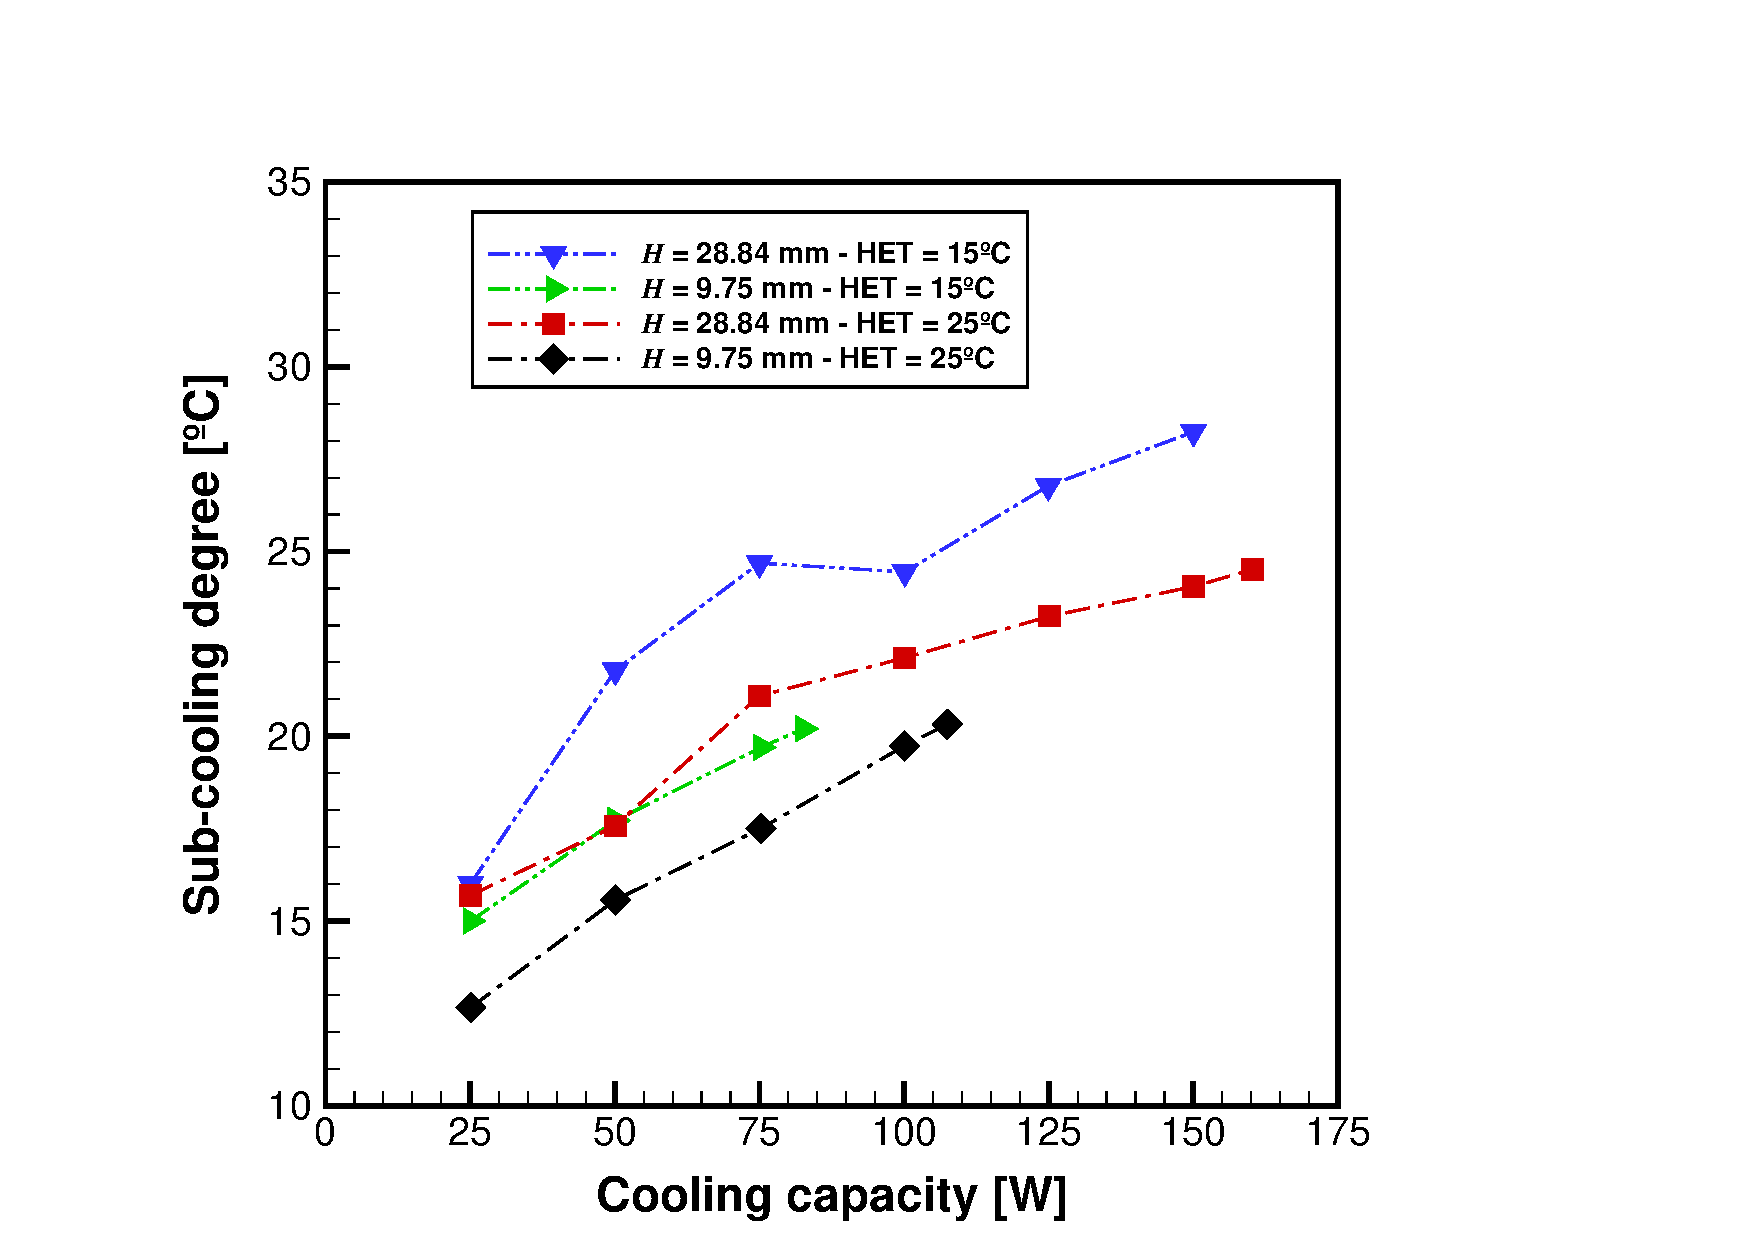
\includegraphics[angle=0,scale=0.325]{Figure_12(b).pdf}}
\caption{(a) Condensing temperature and (b) sub-cooling degree as a function of the applied heat load (cooling capacity) for different jet lengths and hot end temperatures (HET).}
\label{fig:Figure_12}
\end{figure}

\nomenclature[DHET]{HET}{Hot End Temperature}%

The temperature after expansion, i.e., the evaporating temperature, is also higher compared to the test conducted with the lower ambient temperature, for the same cooling capacity. The behavior of $T_{evap}$ is presented in Fig.~\ref{fig:Figure_13} (a). The increase of the saturation temperatures generates a higher pressure lift, which is confirmed by the noticeable increase of the electrical power consumption of the compressor, as depicted in Fig.~\ref{fig:Figure_13} (b).

For the same \textcolor{blue}{jet length}, Fig.~\ref{fig:Figure_14} (a) shows that the surface temperature changes little with the ambient temperature. As the evaporating temperature is observed to increase with an increase in $T_{7}$, the wall superheat becomes lower, which is, essentially, a manifestation of the higher heat transfer coefficient shown in Fig.~\ref{fig:Figure_14} (b). The increase in $\hbar_{s}$ is a  \textcolor{blue}{consequence} of the mass flow rate increase with the cooling capacity as the refrigerant density at the compressor inlet is raised due to the higher evaporating pressures \cite{OliveiraBarbosaJr.2016}.

\begin{figure}[!htp]
\centering
\subfigure[a][]{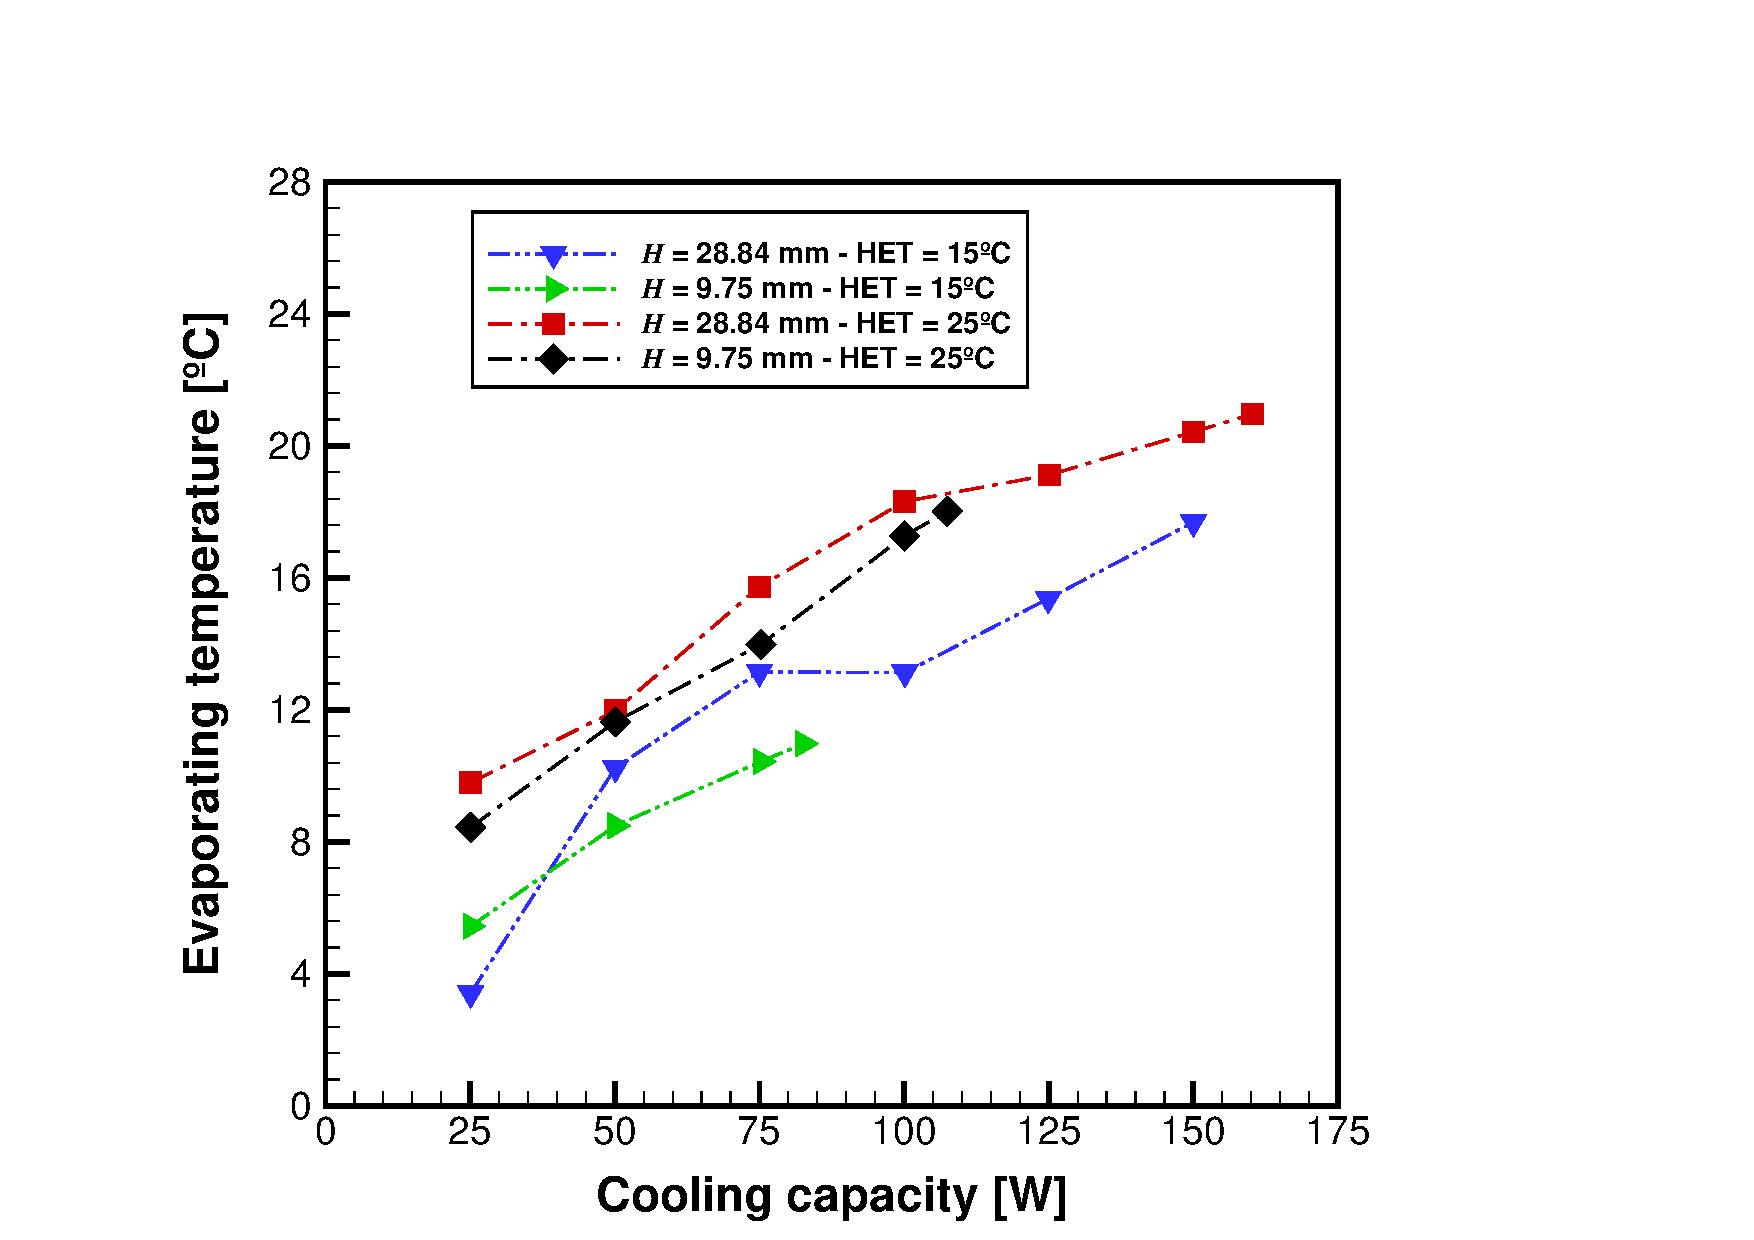
\includegraphics[angle=0,scale=0.325]{Figure_13(a).pdf}}
\hfil
\subfigure[b][]{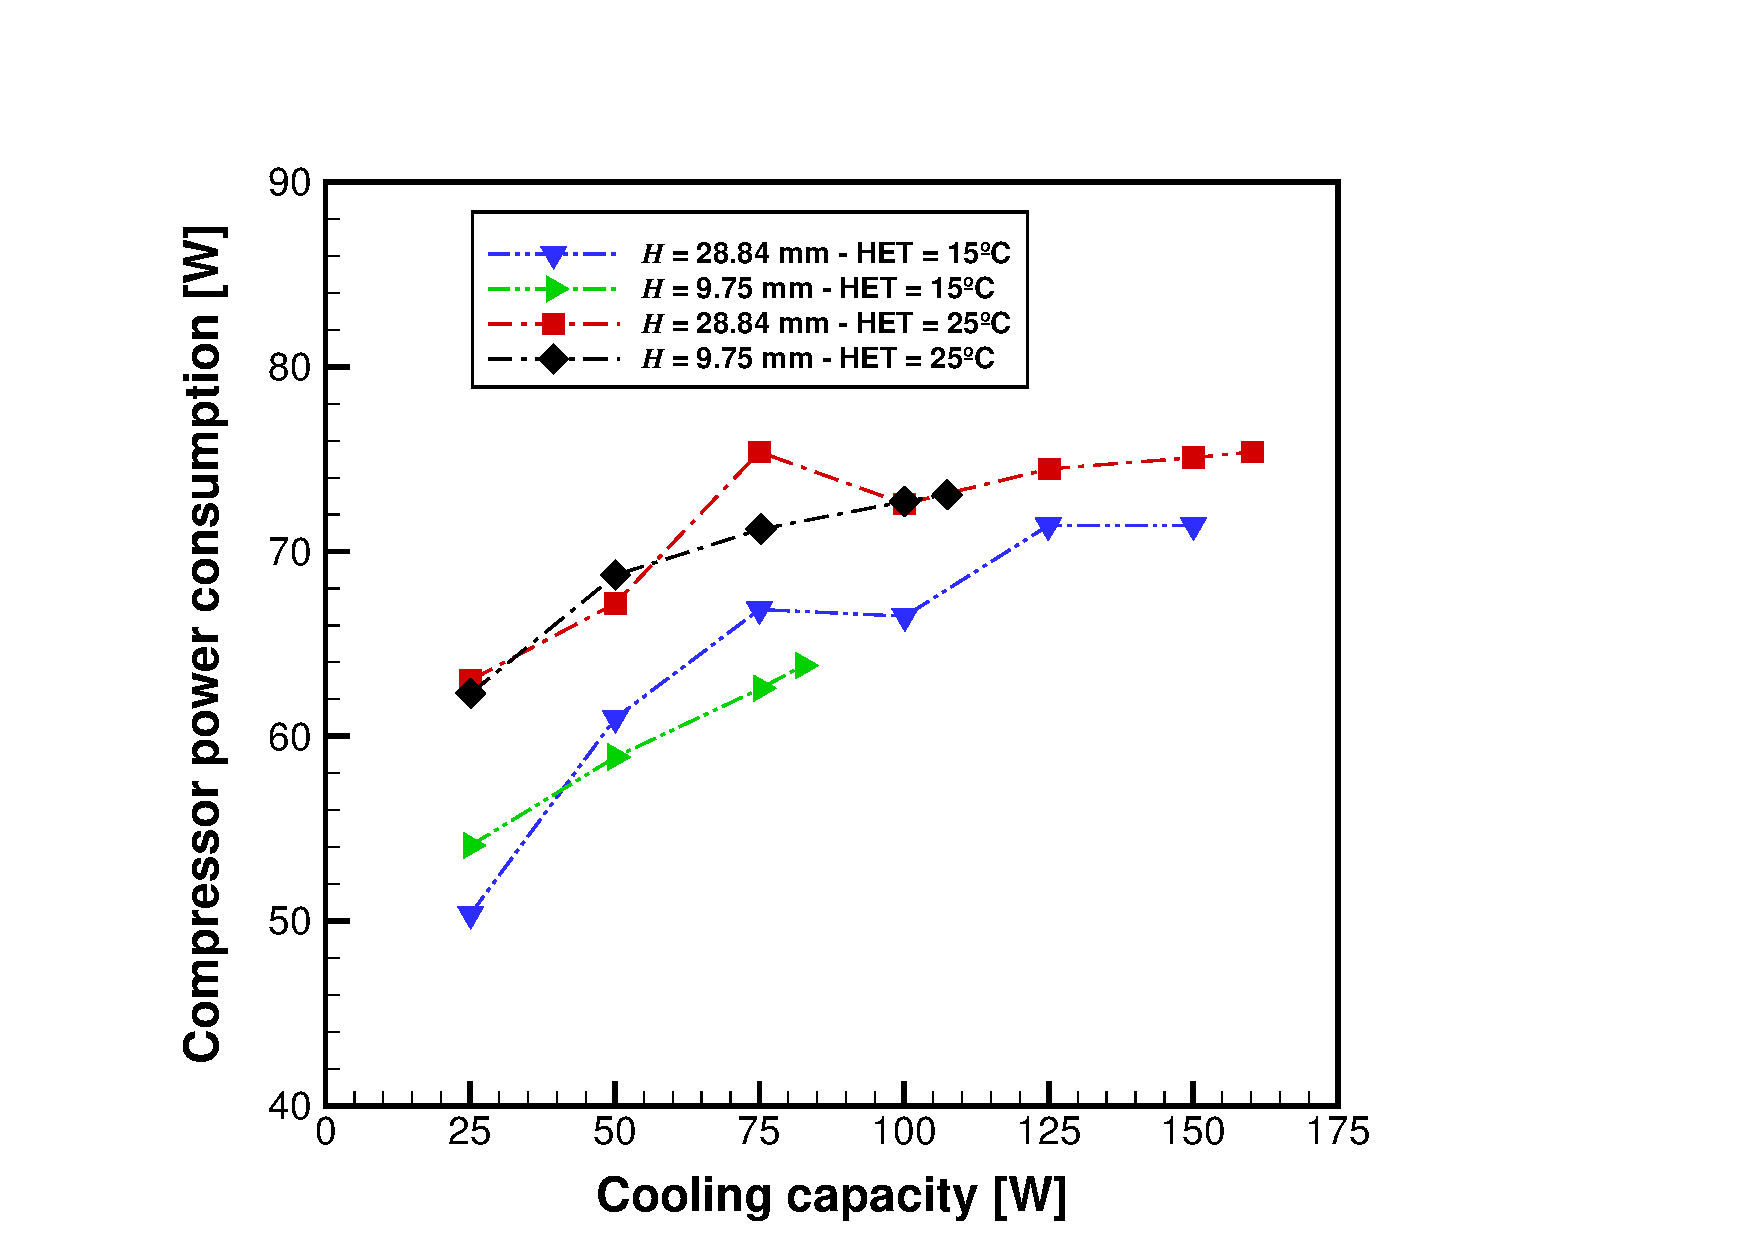
\includegraphics[angle=0,scale=0.325]{Figure_13(b).pdf}}
\caption{(a) Evaporating temperature and (b) compressor power consumption as a function of the applied heat load (cooling capacity) for different jet lengths and hot end temperatures (HET).}
\label{fig:Figure_13}
\end{figure}

\begin{figure}[!htp]
\centering
\subfigure[a][]{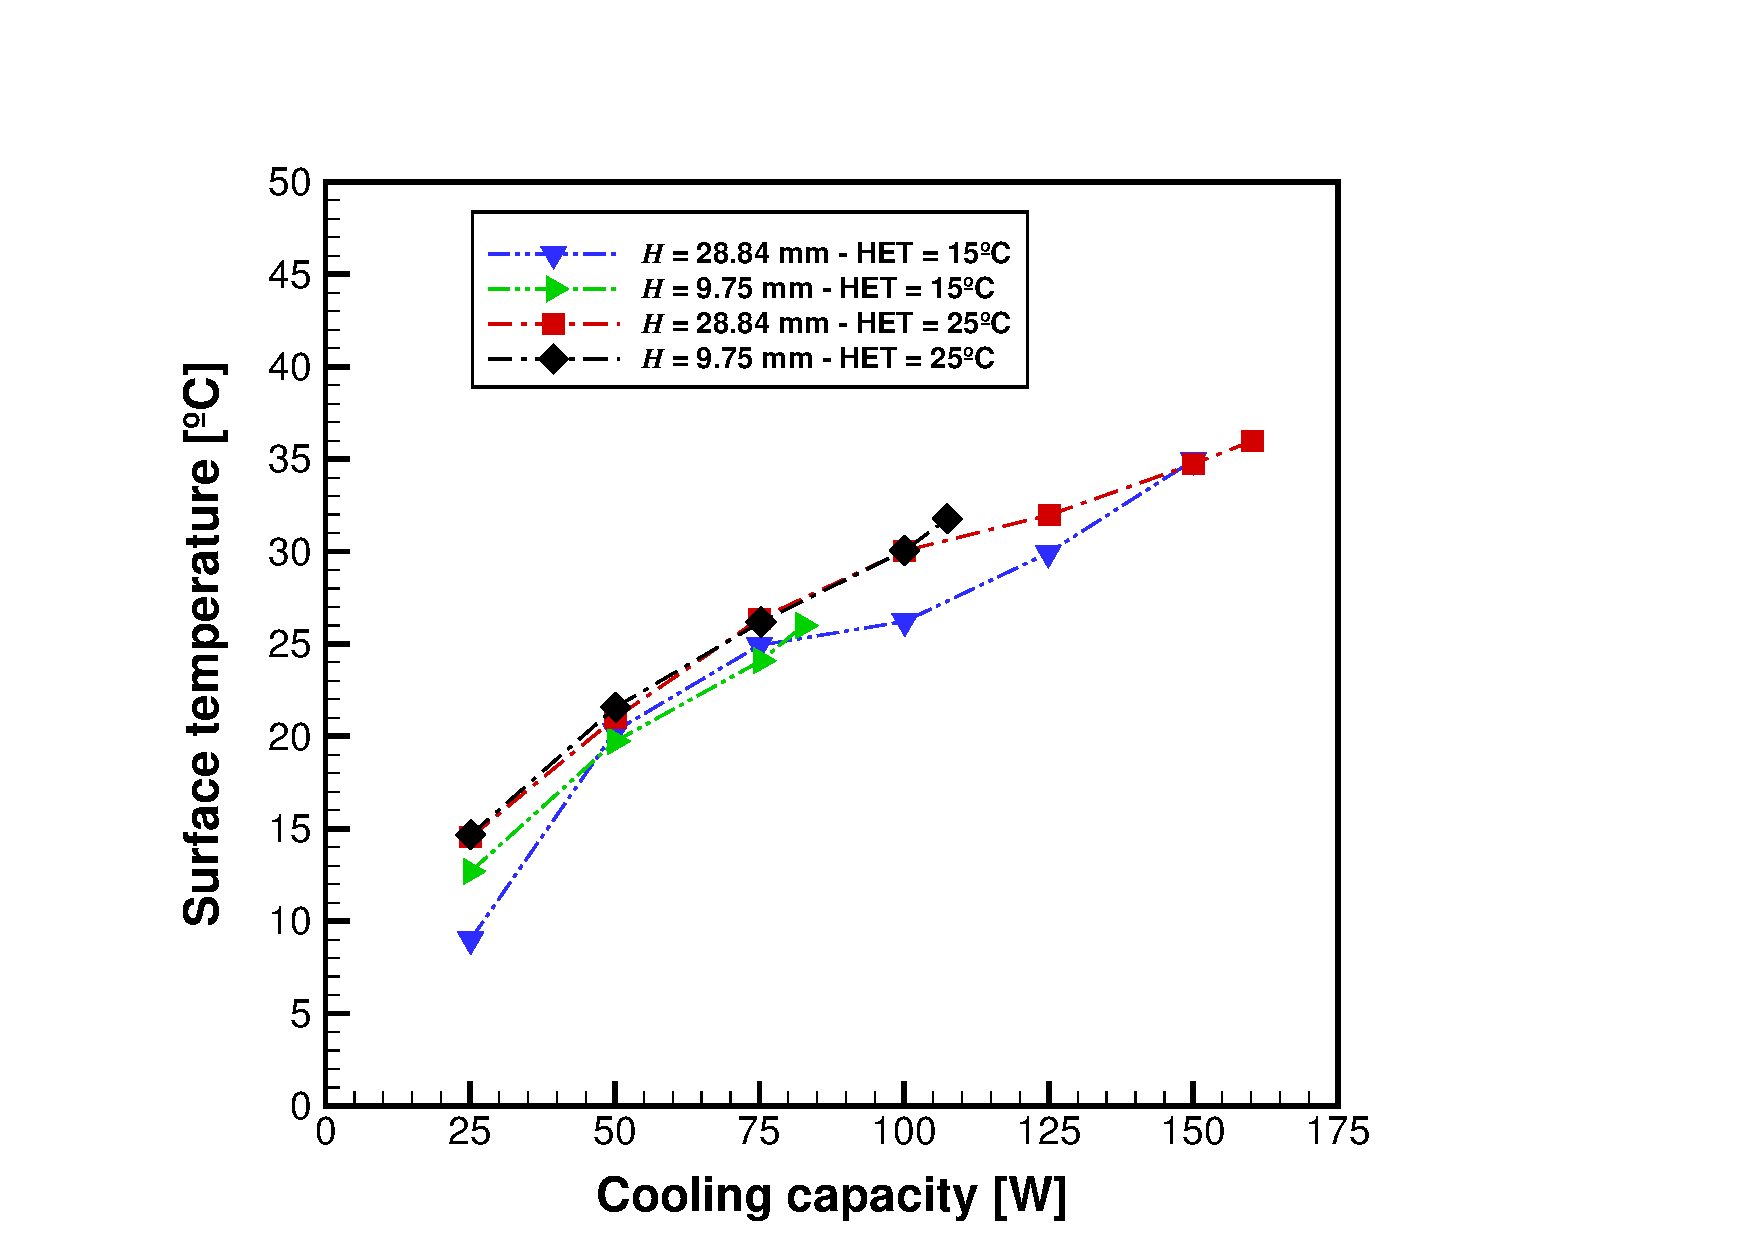
\includegraphics[angle=0,scale=0.325]{Figure_14(a).pdf}}
\hfil
\subfigure[b][]{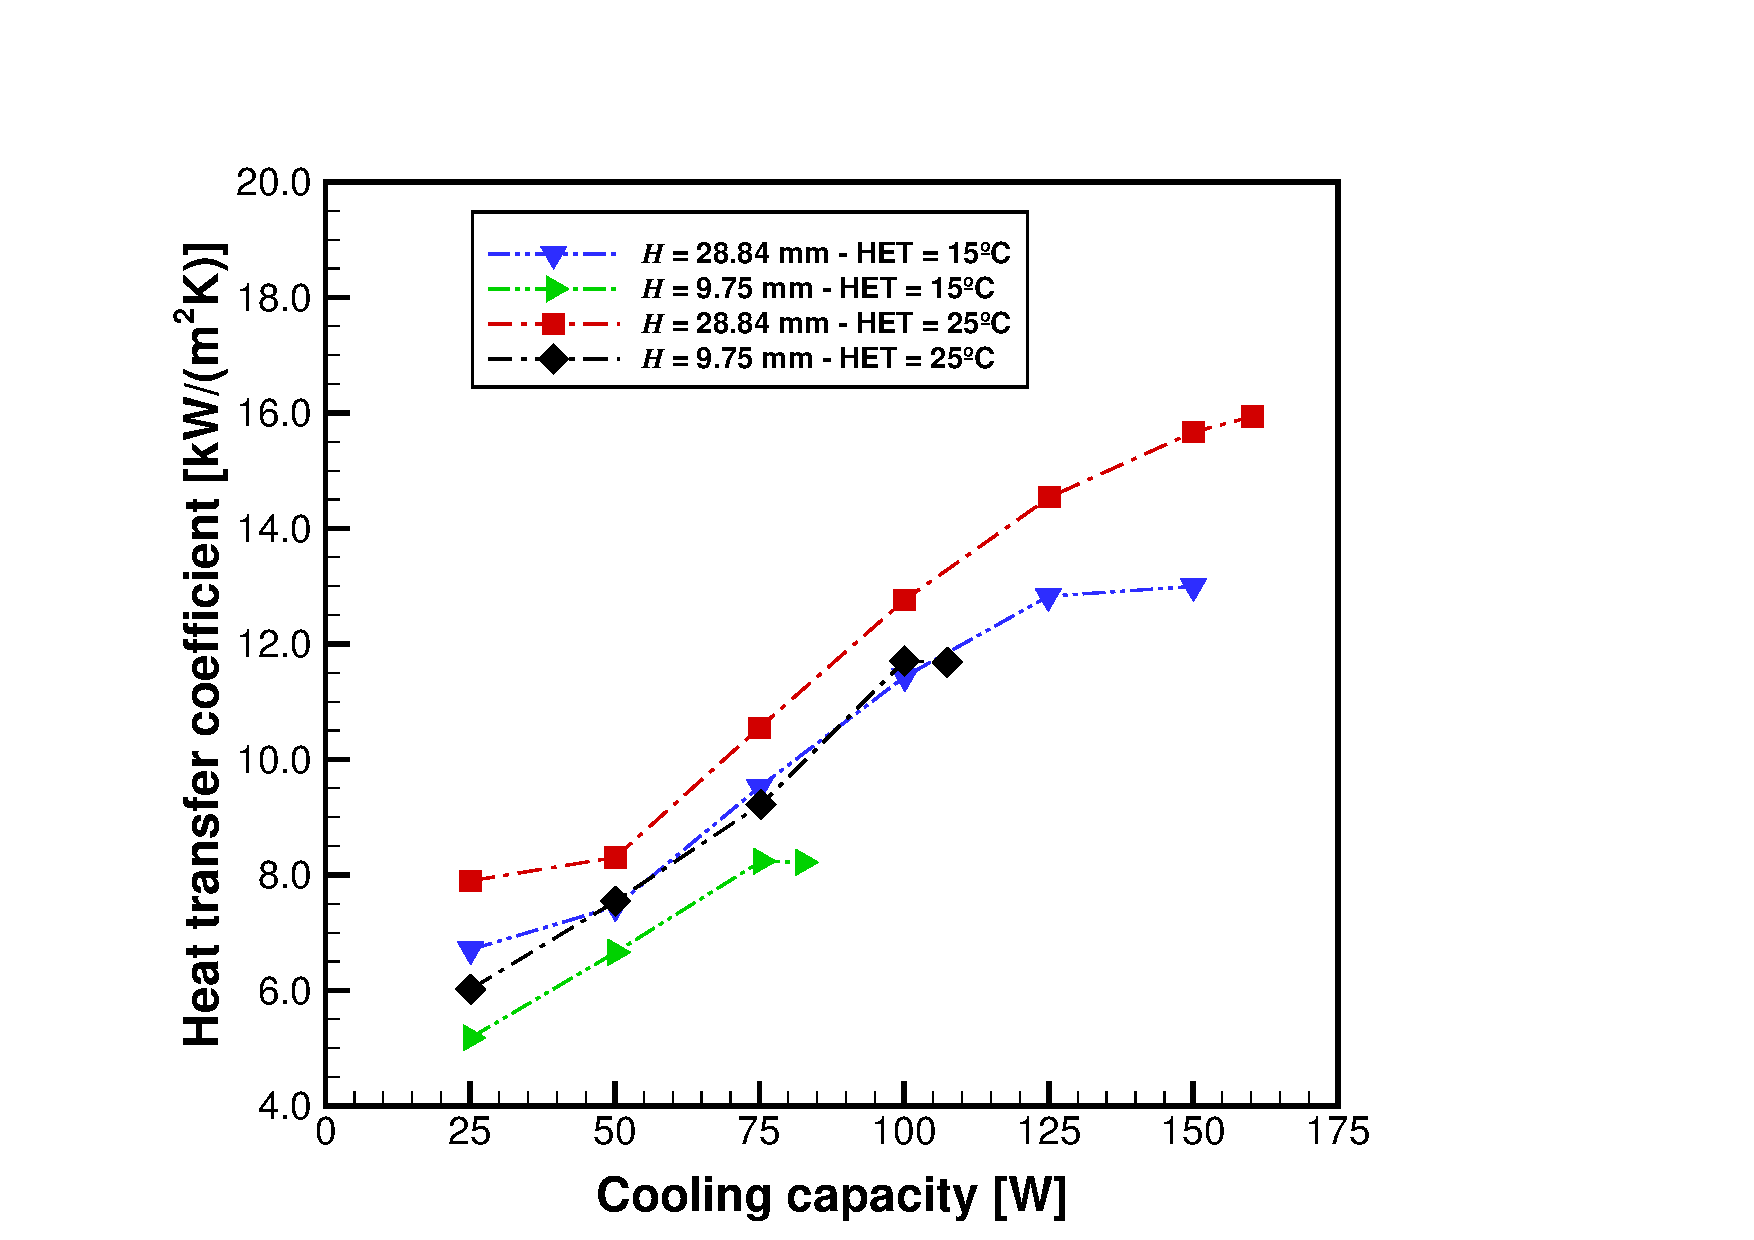
\includegraphics[angle=0,scale=0.325]{Figure_14(b).pdf}}
\caption{(a) Surface temperature and (b) heat transfer coefficient as a function of the applied heat load (cooling capacity) for different jet lengths and hot end temperatures (HET). \colorbox{yellow}{unidades HTC IJR format eixo y}}
\label{fig:Figure_14}
\end{figure}

\section{Conclusions}

A novel two-phase jet heat sink that integrates the evaporator and the expansion device into a single cooling unit has been presented \textcolor{blue}{and evaluated}. The new jet cooler was combined with a compact oil-free linear motor R-134a compressor to demonstrate the applicability of the system in the removal of high heat loads. Experiments have been carried out with a single-orifice configuration of the jet heat sink \textcolor{blue}{(300-$\mu$m diameter)}. %The influence of the following parameters was quantified: (i) compressor piston stroke, (ii) applied thermal load, (iii) orifice-to-heater distance (jet length) and (iv) hot reservoir (ambient) temperature. Heater surface temperature, jet impingement heat transfer coefficient and coefficient of performance were determined. 
 The main conclusions \textcolor{blue}{arising from this work} are as follows:

\begin{enumerate}
\item Reducing the jet length from 28.84 mm to 9.75 mm increased jet splattering and droplet breakup. \textcolor{blue}{This} reduced the heat transfer coefficient and, more significantly, the critical heat flux. However, the impact on the heater surface temperature, compressor power consumption and coefficient of performance was minimal;
\item For a fixed jet length, increasing the hot reservoir temperature from 15\textcelsius\ to 25\textcelsius\ caused an increase in both the evaporating and condensing temperatures. The net effect of this change was an increase of the heat transfer coefficient resulting from the higher mass flow rate. However, as expected, an increase in the compressor power was observed.
\end{enumerate}

\section*{Acknowledgements}

This work was made possible through the financial investment from the EMBRAPII Program (POLO/UFSC EMBRAPII Unit - Emerging Technologies in Cooling and Thermophysics). In addition, financial support from Embraco and from CNPq (Grant No. 573581/2008-8 - National Institute of Science and Technology in Cooling and Thermophysics) is duly acknowledged.

\section*{References}

\bibliographystyle{elsarticle-num}


\bibliography{References(ATE)}

\end{document}